\chapter{视觉、行动与世界模型}\label{chap:world}

\begin{learningbox}
智能体行动于一个不只有语言的世界。本章将介绍基于 Transformer 的模型如何获得语言之外其他模态的世界知识。具体而言，学完本章后，你将能够：
\begin{itemize}[leftmargin=*, nosep]
    \item 描述{\em 视觉语言模型（vision-language model，VLM）}的架构。这类模型通常基于 Transformer，由语言部分与视觉部分组成。视觉语言模型已经取得很大成功，例如生成逼真的虚构图像与短片。

    \item 理解{\em 视觉语言动作模型（vision-language-action model，VLA）}如何工作。这类模型还使用机器人动作进行训练，有助于提高机器人行为的通用性。

    \item 解释智能体为什么能够受益于{\em 世界模型（world model）}：这类模型学到了周围世界的一些物理属性，使智能体不至于尝试穿墙而过。
\end{itemize}
\end{learningbox}

\section{多模态视觉语言模型}\label{sec:vlm}

许多决策都涉及视觉。本节将介绍，Transformer 架构同样能够学习词元化的视觉模式。在语言数据与视觉数据上共同预训练的模型，称为视觉语言模型。它们通常包含 (1) 语言部分，(2) 视觉部分，以及 (3) 结合这两类嵌入的部分。

我们将讨论视觉语言模型的不同架构。对于每类模型，分别介绍其任务、模型架构与训练算法，并看到一些令人印象深刻的结果。

计算机视觉在人工智能中有着悠久而成功的历史。早在自然语言处理取得突破之前，深度学习就已在图像识别任务中取得成功 \citep{krizhevsky2012imagenet}。这两个成功的领域能否结合起来？这不是一个简单的问题，因为二者依托的深度学习架构颇不相同：图像处理以卷积神经网络为基础，擅长处理由像素组成的二维矩形网格；语言处理则以 Transformer 为基础，擅长处理一维词元序列。

正如下面将看到的，人们确实已经开发出结合这两个领域的架构，如今大多数前沿模型都已成为视觉语言模型。

\begin{figure}
  \begin{center}
    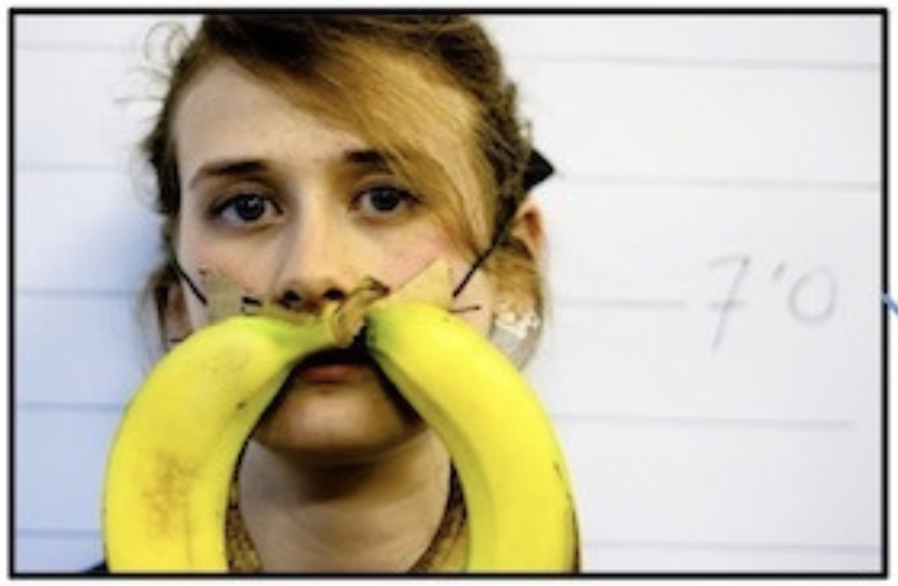
\includegraphics[width=7cm]{figures/VQAbanana}
    \caption{视觉问答任务中的问题可能是：{\em 这副胡子是用什么做的？}} \label{fig:vqa}
  \end{center}
\end{figure}

\subsection{任务}
先来讨论视觉语言模型需要解决哪些类型的任务，并列举一些常见的基准测试套件。在理解方面，可以通过视觉问答（visual question answering，VQA）任务，检验模型是否获得了对视觉图像的某种文本理解。相关的生成任务是图像描述：模型需要为图像生成文字说明。此外，模型也可能承担图像生成任务。

来看几个任务示例。针对图~\ref{fig:vqa}，视觉问答问题可以是“{\em 这副胡子是用什么做的？}”，系统应回答“{\em 香蕉}”。另一类典型问题，是统计图像特定区域中某种颜色、某种形状的物体数量，例如回答“{\em 这个场景中，桌子的上方角落有没有一个红色方块？}”。任务可以非常多样，常见基准测试包括 MOSAIC \citep{burda2025culturally}、GLOBAL-RG \citep{bhatia2024local}、CultureVQA \citep{nayak2024benchmarking}、FoodieQA \citep{li2024foodieqa} 与 MaRVL \citep{liu2021visually}。

\begin{figure}
  \begin{center}
    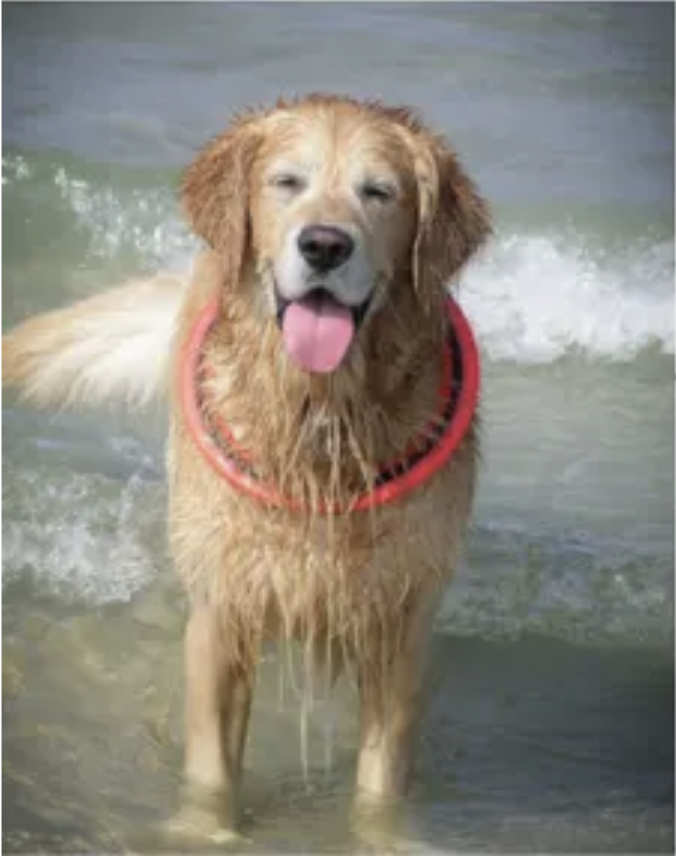
\includegraphics[width=6cm]{figures/captioning}
    \caption{图像描述任务，一种可能的描述是：{\em 一只开心的狗站在海水中。}} \label{fig:cap}
  \end{center}
\end{figure}

在图像描述问题中，可以提示模型为图~\ref{fig:cap}~中的场景生成说明，图中是{\em 一只站在海水中的开心的狗}。需要注意，其他表述也可能同样成立，例如{\em 一只湿漉漉的狗}、{\em 一只感到寒冷的狗}，或{\em 一只戴着红色项圈、站在海水中的狗}。常见基准测试包括 MS-COCO \citep{lin2014microsoft}、nocaps，\footnote{\url{https://nocaps.org}}以及面向视频、采用传统短描述评估的 MSR-VTT \citep{xu2016msr} 与 VATEX \citep{wang2019vatex}。较新的基准测试开始关注详细、多方面的描述，包括 DetailCaps \citep{dong2024benchmarking}、VDC \citep{chai2024auroracap} 与 CapArena \citep{cheng2025caparena}。

视觉语言模型的典型应用包括摘要、图像生成、搜索与检索、图像分割，以及目标检测。面向专家级通用人工智能的大规模多学科多模态理解与推理基准测试（Massive Multi-discipline Multi-modal Understanding and Reasoning Benchmark，MMMU），是视觉语言模型的一项综合性基准测试 \citep{yue2024mmmu}。

\subsection{架构}
了解了视觉语言模型接受测试的任务类型后，我们该如何设计能够完成这些任务的模型？

将语言建模为词元序列时，它属于一维的序列问题领域；将视觉建模为像素网格时，它属于二维的矩形问题领域。相应地，两类应用采用不同的深度学习架构：语言使用 Transformer 架构寻找序列模式，图像使用卷积神经网络寻找二维模式。因此，多模态视觉语言模型应当采用何种架构，并不显而易见。事实上，最初人们甚至不清楚视觉语言模型究竟能否工作。

研究首先关注一个问题：除了传统的卷积神经网络（convolutional neural network，CNN），Transformer 架构能否也用于图像处理？为此，人们开发了专门的视觉 Transformer 与词元化方案，并在图像处理中取得良好效果 \citep{dosovitskiy2020image}。

\begin{figure}
    \centering
    % 依据原包 vlm.png；保留四个视觉词元、四个文本词元及其汇合关系。
\begin{tikzpicture}[font=\small,box/.style={rounded corners=4pt,fill=green!20,minimum height=.8cm,align=center},flow/.style={-{Stealth[length=2.5mm]},line width=1pt,draw=gray!80!black}]
\node[box,minimum width=9cm] (dec) at (4.5,3.8) {文本解码器};
\node[align=center] at (4.5,2.4) {投影后的视觉词元与文本嵌入词元拼接};
\foreach \xx in {0.4,1.5,2.6,3.7}{\node[rounded corners=3pt,fill=yellow!35,minimum width=.7cm,minimum height=.3cm] at (\xx,1.9) {};}
\foreach \xx in {5.0,6.1,7.2,8.3}{\node[rounded corners=3pt,fill=red!10,minimum width=.7cm,minimum height=.3cm] at (\xx,1.9) {};}
\node[box,minimum width=4cm] (proj) at (2.1,0) {多模态投影器};
\node (txt) at (6.7,0) {文本嵌入};
\draw[flow] (proj.north) -- (2.1,1.3);
\draw[flow] (txt.north) -- (6.7,1.3);
\draw[flow] (4.5,2.9) -- (dec.south);
\end{tikzpicture}

    \caption{视觉语言模型架构，依据 LLaVa \citep{liu2023visual} 绘制，原图来自 Huggingface。}
    \label{fig:vlm}
\end{figure}

\begin{figure}
    \centering
    % 保留原始面板、实拍、示例与全部连线；仅以 TikZ 覆盖说明标签。
\begin{tikzpicture}
\node[anchor=south west,inner sep=0] (im) at (0,0) {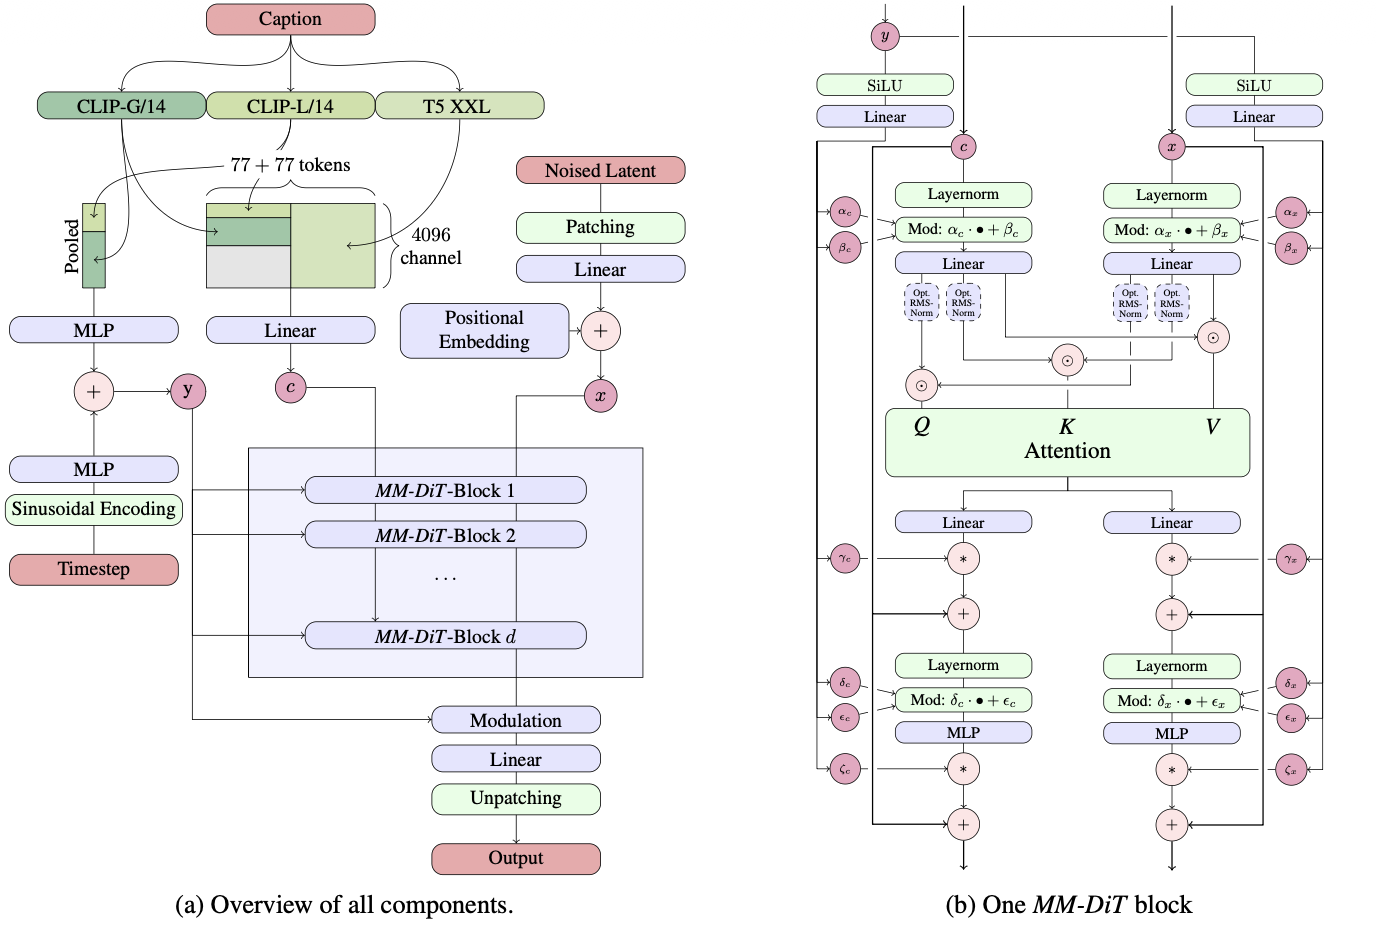
\includegraphics[width=\linewidth]{figures/stable.png}};
\begin{scope}[x={(im.south east)},y={(im.north west)}]
\fill[red!15] (0.153343,0.968017) rectangle (0.270349,0.992537);
\node[align=center,inner sep=0pt,font=\fontsize{8}{9}\selectfont,text width=0.117006\linewidth,rotate=0] at (0.211846,0.980277) {图像描述};
\fill[white] (0.159884,0.811301) rectangle (0.260901,0.837953);
\node[align=center,inner sep=0pt,font=\fontsize{7.5}{8.5}\selectfont,text width=0.101017\linewidth,rotate=0] at (0.210392,0.824627) {77 + 77 词元};
\fill[white] (0.287064,0.708955) rectangle (0.339390,0.764392);
\node[align=center,inner sep=0pt,font=\fontsize{7.5}{8.5}\selectfont,text width=0.052326\linewidth,rotate=0] at (0.313227,0.736674) {4096\\通道};
\fill[red!15] (0.378634,0.807036) rectangle (0.494913,0.831557);
\node[align=center,inner sep=0pt,font=\fontsize{8}{9}\selectfont,text width=0.116279\linewidth,rotate=0] at (0.436773,0.819296) {加噪潜变量};
\fill[green!8] (0.378634,0.745203) rectangle (0.494186,0.769723);
\node[align=center,inner sep=0pt,font=\fontsize{8}{9}\selectfont,text width=0.115552\linewidth,rotate=0] at (0.436410,0.757463) {分块};
\fill[blue!8] (0.378634,0.701493) rectangle (0.494186,0.726013);
\node[align=center,inner sep=0pt,font=\fontsize{8}{9}\selectfont,text width=0.115552\linewidth,rotate=0] at (0.436410,0.713753) {线性层};
\fill[blue!8] (0.295785,0.624733) rectangle (0.408430,0.672708);
\node[align=center,inner sep=0pt,font=\fontsize{8}{9}\selectfont,text width=0.112645\linewidth,rotate=0] at (0.352108,0.648721) {位置嵌入};
\fill[green!8] (0.007267,0.442431) rectangle (0.129360,0.470149);
\node[align=center,inner sep=0pt,font=\fontsize{7.5}{8.5}\selectfont,text width=0.122093\linewidth,rotate=0] at (0.068314,0.456290) {正弦编码};
\fill[red!15] (0.010174,0.380597) rectangle (0.125000,0.406183);
\node[align=center,inner sep=0pt,font=\fontsize{8}{9}\selectfont,text width=0.114826\linewidth,rotate=0] at (0.067587,0.393390) {时间步};
\fill[blue!8] (0.226017,0.465885) rectangle (0.421512,0.488273);
\node[align=center,inner sep=0pt,font=\fontsize{8}{9}\selectfont,text width=0.195494\linewidth,rotate=0] at (0.323765,0.477079) {MM-DiT 块 1};
\fill[blue!8] (0.226017,0.416844) rectangle (0.421512,0.439232);
\node[align=center,inner sep=0pt,font=\fontsize{8}{9}\selectfont,text width=0.195494\linewidth,rotate=0] at (0.323765,0.428038) {MM-DiT 块 2};
\fill[blue!8] (0.226017,0.308102) rectangle (0.421512,0.330490);
\node[align=center,inner sep=0pt,font=\fontsize{8}{9}\selectfont,text width=0.195494\linewidth,rotate=0] at (0.323765,0.319296) {MM-DiT 块 d};
\fill[blue!8] (0.317587,0.221748) rectangle (0.431686,0.243070);
\node[align=center,inner sep=0pt,font=\fontsize{8}{9}\selectfont,text width=0.114099\linewidth,rotate=0] at (0.374637,0.232409) {调制};
\fill[blue!8] (0.317587,0.178038) rectangle (0.431686,0.199360);
\node[align=center,inner sep=0pt,font=\fontsize{8}{9}\selectfont,text width=0.114099\linewidth,rotate=0] at (0.374637,0.188699) {线性层};
\fill[green!8] (0.317587,0.135394) rectangle (0.431686,0.156716);
\node[align=center,inner sep=0pt,font=\fontsize{8}{9}\selectfont,text width=0.114099\linewidth,rotate=0] at (0.374637,0.146055) {还原分块};
\fill[red!15] (0.317587,0.072495) rectangle (0.431686,0.093817);
\node[align=center,inner sep=0pt,font=\fontsize{8}{9}\selectfont,text width=0.114099\linewidth,rotate=0] at (0.374637,0.083156) {输出};
\fill[white] (0.039971,0.696162) rectangle (0.060320,0.771855);
\node[align=center,inner sep=0pt,font=\fontsize{6.5}{7.5}\selectfont,text width=0.020349\linewidth,rotate=0] at (0.050145,0.734009) {池\\化};
\fill[blue!8] (0.596657,0.868870) rectangle (0.691134,0.884861);
\node[align=center,inner sep=0pt,font=\fontsize{7.5}{8.5}\selectfont,text width=0.094477\linewidth,rotate=0] at (0.643895,0.876866) {线性层};
\fill[blue!8] (0.864826,0.868870) rectangle (0.956395,0.884861);
\node[align=center,inner sep=0pt,font=\fontsize{7.5}{8.5}\selectfont,text width=0.091570\linewidth,rotate=0] at (0.910610,0.876866) {线性层};
\fill[blue!8] (0.654797,0.711087) rectangle (0.747820,0.728145);
\node[align=center,inner sep=0pt,font=\fontsize{7.5}{8.5}\selectfont,text width=0.093023\linewidth,rotate=0] at (0.701308,0.719616) {线性层};
\fill[blue!8] (0.805959,0.711087) rectangle (0.899709,0.728145);
\node[align=center,inner sep=0pt,font=\fontsize{7.5}{8.5}\selectfont,text width=0.093750\linewidth,rotate=0] at (0.852834,0.719616) {线性层};
\fill[blue!8] (0.654797,0.433902) rectangle (0.747820,0.450959);
\node[align=center,inner sep=0pt,font=\fontsize{7.5}{8.5}\selectfont,text width=0.093023\linewidth,rotate=0] at (0.701308,0.442431) {线性层};
\fill[blue!8] (0.805959,0.433902) rectangle (0.899709,0.450959);
\node[align=center,inner sep=0pt,font=\fontsize{7.5}{8.5}\selectfont,text width=0.093750\linewidth,rotate=0] at (0.852834,0.442431) {线性层};
\fill[green!8] (0.651163,0.777186) rectangle (0.750727,0.805970);
\node[align=center,inner sep=0pt,font=\fontsize{7.5}{8.5}\selectfont,text width=0.099564\linewidth,rotate=0] at (0.700945,0.791578) {层归一化};
\fill[green!8] (0.803052,0.777186) rectangle (0.902616,0.805970);
\node[align=center,inner sep=0pt,font=\fontsize{7.5}{8.5}\selectfont,text width=0.099564\linewidth,rotate=0] at (0.852834,0.791578) {层归一化};
\fill[green!8] (0.651163,0.276119) rectangle (0.750727,0.304904);
\node[align=center,inner sep=0pt,font=\fontsize{7.5}{8.5}\selectfont,text width=0.099564\linewidth,rotate=0] at (0.700945,0.290512) {层归一化};
\fill[green!8] (0.803052,0.276119) rectangle (0.902616,0.304904);
\node[align=center,inner sep=0pt,font=\fontsize{7.5}{8.5}\selectfont,text width=0.099564\linewidth,rotate=0] at (0.852834,0.290512) {层归一化};
\fill[green!8] (0.652616,0.742004) rectangle (0.686047,0.769723);
\node[align=center,inner sep=0pt,font=\fontsize{6}{7}\selectfont,text width=0.033430\linewidth,rotate=0] at (0.669331,0.755864) {调制};
\fill[green!8] (0.803779,0.742004) rectangle (0.837209,0.769723);
\node[align=center,inner sep=0pt,font=\fontsize{6}{7}\selectfont,text width=0.033430\linewidth,rotate=0] at (0.820494,0.755864) {调制};
\fill[green!8] (0.652616,0.240938) rectangle (0.686047,0.268657);
\node[align=center,inner sep=0pt,font=\fontsize{6}{7}\selectfont,text width=0.033430\linewidth,rotate=0] at (0.669331,0.254797) {调制};
\fill[green!8] (0.803779,0.240938) rectangle (0.837209,0.268657);
\node[align=center,inner sep=0pt,font=\fontsize{6}{7}\selectfont,text width=0.033430\linewidth,rotate=0] at (0.820494,0.254797) {调制};
\fill[blue!5] (0.656977,0.656716) rectangle (0.682413,0.699360);
\node[align=center,inner sep=0pt,font=\fontsize{5}{6}\selectfont,text width=0.025436\linewidth,rotate=0] at (0.669695,0.678038) {RMS};
\fill[blue!5] (0.689680,0.656716) rectangle (0.715116,0.699360);
\node[align=center,inner sep=0pt,font=\fontsize{5}{6}\selectfont,text width=0.025436\linewidth,rotate=0] at (0.702398,0.678038) {RMS};
\fill[blue!5] (0.808140,0.656716) rectangle (0.833576,0.699360);
\node[align=center,inner sep=0pt,font=\fontsize{5}{6}\selectfont,text width=0.025436\linewidth,rotate=0] at (0.820858,0.678038) {RMS};
\fill[blue!5] (0.840116,0.656716) rectangle (0.865552,0.699360);
\node[align=center,inner sep=0pt,font=\fontsize{5}{6}\selectfont,text width=0.025436\linewidth,rotate=0] at (0.852834,0.678038) {RMS};
\fill[green!8] (0.739099,0.503198) rectangle (0.820494,0.529851);
\node[align=center,inner sep=0pt,font=\fontsize{8}{9}\selectfont,text width=0.081395\linewidth,rotate=0] at (0.779797,0.516525) {注意力};
\fill[white] (0.123547,0.007463) rectangle (0.474564,0.050107);
\node[align=center,inner sep=0pt,font=\fontsize{8.5}{9.5}\selectfont,text width=0.351017\linewidth,rotate=0] at (0.299055,0.028785) {（a）全部组件概览};
\fill[white] (0.650436,0.001066) rectangle (0.987645,0.050107);
\node[align=center,inner sep=0pt,font=\fontsize{7.5}{8.5}\selectfont,text width=0.337209\linewidth,rotate=0] at (0.819041,0.025586) {（b）一个 MM-DiT 块\\虚线小框：可选 RMS 归一化};
\fill[blue!8] (0.153343,0.636461) rectangle (0.268895,0.660981);
\node[align=center,inner sep=0pt,font=\fontsize{8}{9}\selectfont,text width=0.115552\linewidth] at (0.211119,0.648721) {线性层};
\end{scope}
\end{tikzpicture}

    \caption{Stable Diffusion 架构 \citep{esser2024scaling}。}
    \label{fig:stable}
\end{figure}

接下来，需要一种架构来结合语言嵌入与图像嵌入，并生成语言。一般而言，视觉语言模型包含一个图像编码器，可以是卷积神经网络，也可以是采用专门词元化方式的视觉 Transformer，以及一个文本编码器。二者连接到嵌入投影器，以对齐图像与文本表示；投影器通常是稠密神经网络，最后再连接文本解码器，即 Transformer。图~\ref{fig:vlm}~以 LLaVa 为例，展示了这种架构 \citep{liu2023visual}。视觉嵌入与文本嵌入之间，通过一个将视觉嵌入投影为另一种嵌入的网络建立联系，使模型能够进行统一推理。投影网络通常是稠密神经网络，即多层感知机。

人们还开发了更复杂的架构，最先进的视觉语言模型可以包含多个 Transformer 模块，结构相当复杂。例如，图~\ref{fig:stable}~展示了生成式 Stable Diffusion 架构 \citep{esser2024scaling,weng2021diffusion,yang2023diffusion}。

\subsection{学习算法}
介绍了视觉语言模型的任务与架构后，现在来看模型所使用的学习算法。不同的编码器与投影器，使视觉语言模型能够接受训练。训练算法应当对齐并融合视觉编码器与语言编码器中的知识。这样，模型就可以关联图像信息与文本信息，分析查询，并依据两种模态给出回答。文献中已经提出了多种训练视觉语言模型的方法。

OpenAI 的 CLIP \citep{radford2021learning}，全称为{\em 对比式语言—图像预训练}，采用对比学习（contrastive learning）。对比学习是一种自监督学习方法，在数据集没有相应标签时构造监督信号。其思想是在嵌入空间中，把不相似的数据点推远，把相似数据点拉近。对比学习最大化{\em 正样本}对的表示相似度，例如同一图像的相似形式；同时最小化{\em 负样本}对的相似度，例如不同物体的图像。

另一种方法是掩码。与语言模型训练中的用法相同，视觉语言模型学习预测输入文本或图像中随机遮住的部分。例如，给定一段未遮蔽的图像描述，模型学习重建图像中隐藏的像素。FLAVA 是一个例子，其全称为{\em 基础语言与视觉对齐（foundational language and vision alignment）}，采用视觉 Transformer 作为图像编码器，并采用 Transformer 作为语言编码器与多模态投影器 \citep{singh2022flava}。

\begin{figure}
    \centering
    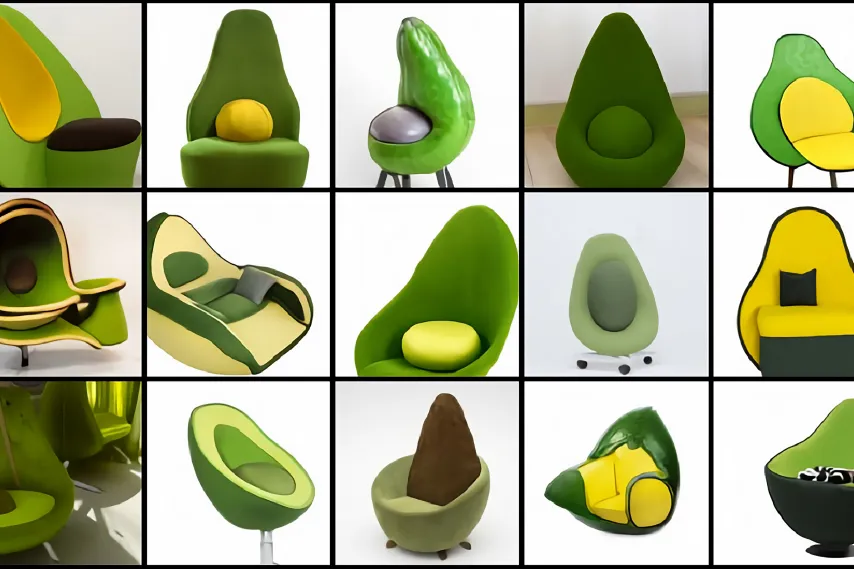
\includegraphics[width=\linewidth]{figures/dalle}
    \caption{DALL-E：牛油果扶手椅}
    \label{fig:dalle}
\end{figure}
视觉语言模型也可以采用生成式用法，根据文本提示生成图像。流行的文生图模型通常使用扩散模型 \citep{ho2022large,yang2023diffusion}。著名例子包括 Google 的 Imagen \citep{baldridge2024imagen}、Midjourney、OpenAI 的 DALL-E \citep{betker2023improving}，以及 Stability AI 的 Stable Diffusion \citep{esser2024scaling}。DALL-E 2 使用以 CLIP 图像嵌入为条件的扩散模型。图~\ref{fig:dalle}~展示了 DALL-E 著名的超现实牛油果扶手椅。

从零开始预训练视觉语言模型的成本很高。由于这类模型由语言模型与视觉模型组成，我们可以尝试用一个或两个已经预训练过的现成模型，构建视觉语言模型。既可以使用预训练大语言模型，也可以使用预训练视觉编码器，再添加映射网络，将视觉嵌入投影到语言模型的文本输入空间。LLaVA 是一个例子，全称为{\em 大型语言与视觉助手（large language and vision assistant）}。它采用 Vicuna 语言解码器与 CLIP ViT 视觉编码器，通过线性投影器，把两者输出合并到一个维数相同的共享空间 \citep{liu2023visual}。

如今已经开发出许多视觉语言模型。它们在基准任务上通常表现良好，也经常用于智能体决策。视觉语言模型已经非常普及，当前许多开放与商业大语言模型都属于这一类，例如 DeepSeek-VL2、Gemini 2.0 Flash、GPT-4o、Llama 3.2、NVLM 与 Qwen 2.5-VL。

\begin{figure}
    \centering
    % 八个数据集名与八幅原图不变；只替换下方自然语言描述。
\begin{tikzpicture}
\node[anchor=south west,inner sep=0] (im) at (0,0) {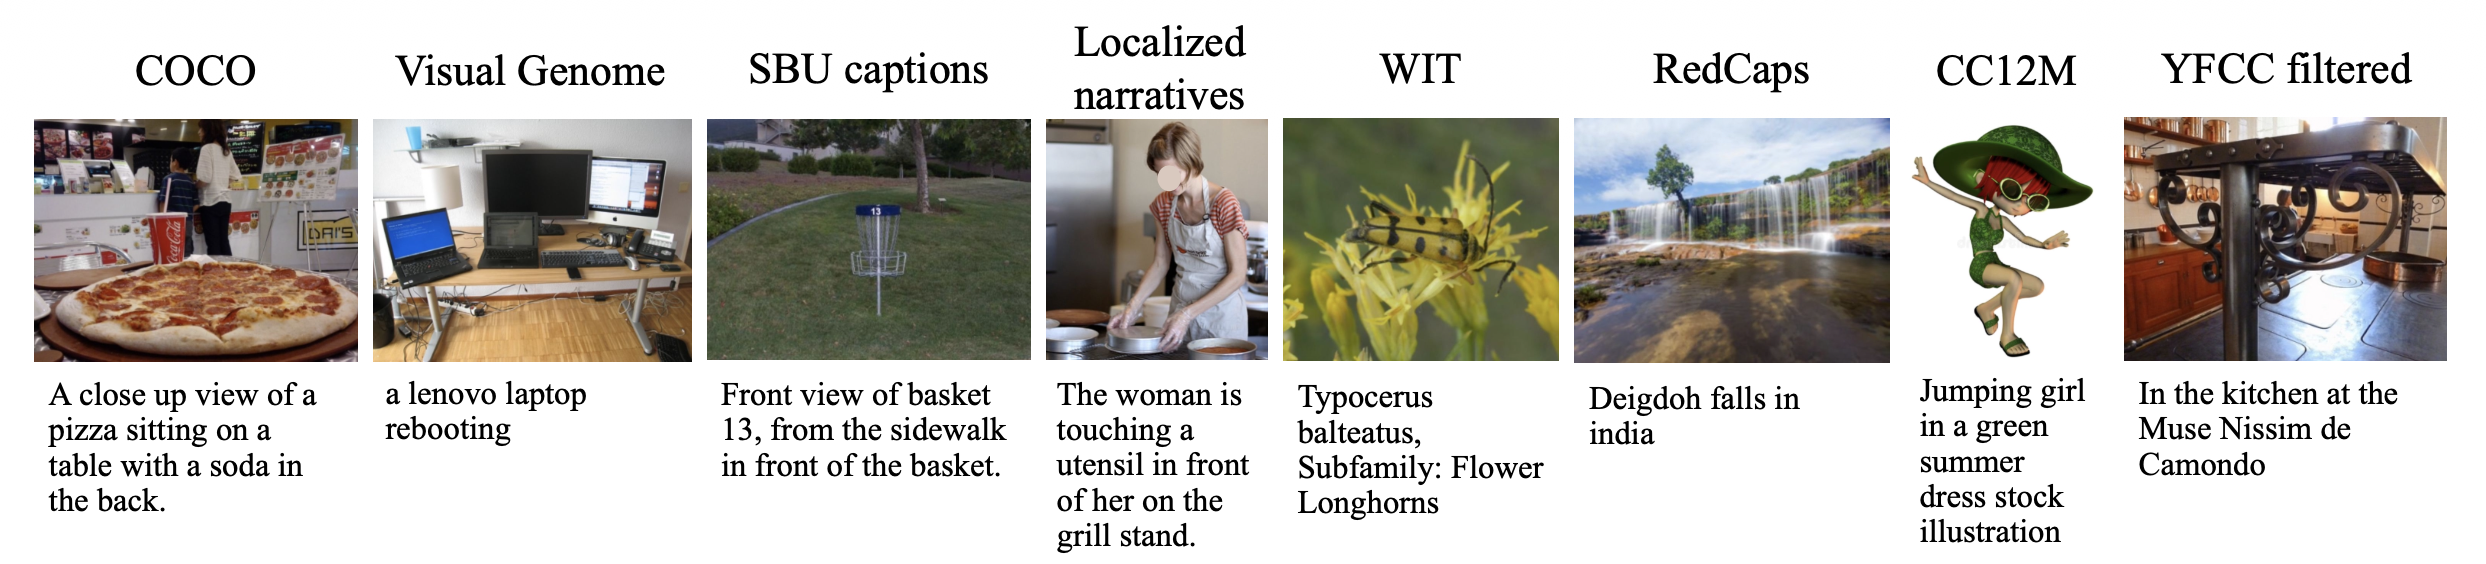
\includegraphics[width=\linewidth]{figures/flava.png}};
\begin{scope}[x={(im.south east)},y={(im.north west)}]
\fill[white] (0,0) rectangle (1,.337);
\node[anchor=north west,align=left,inner sep=0pt,text width=.113\linewidth,font=\fontsize{7}{8.5}\selectfont] at (.013,.323) {桌上一份披萨的特写，后方放着一杯汽水。};
\node[anchor=north west,align=left,inner sep=0pt,text width=.113\linewidth,font=\fontsize{7}{8.5}\selectfont] at (.154,.323) {一台正在重新启动的 Lenovo 笔记本电脑。};
\node[anchor=north west,align=left,inner sep=0pt,text width=.113\linewidth,font=\fontsize{7}{8.5}\selectfont] at (.291,.323) {从篮筐前的人行道正面看 13 号篮筐。};
\node[anchor=north west,align=left,inner sep=0pt,text width=.087\linewidth,font=\fontsize{7}{8.5}\selectfont] at (.425,.323) {女子正在触碰她面前烤架上的一件器具。};
\node[anchor=north west,align=left,inner sep=0pt,text width=.103\linewidth,font=\fontsize{7}{8.5}\selectfont] at (.523,.323) {\textit{Typocerus balteatus}，亚科：花天牛。};
\node[anchor=north west,align=left,inner sep=0pt,text width=.113\linewidth,font=\fontsize{7}{8.5}\selectfont] at (.640,.323) {印度的 Deigdoh 瀑布。};
\node[anchor=north west,align=left,inner sep=0pt,text width=.078\linewidth,font=\fontsize{7}{8.5}\selectfont] at (.773,.323) {身穿绿色夏季连衣裙、跃起的女孩，素材插画。};
\node[anchor=north west,align=left,inner sep=0pt,text width=.122\linewidth,font=\fontsize{7}{8.5}\selectfont] at (.862,.323) {在 Muse Nissim de Camondo 博物馆的厨房中。};
\end{scope}
\end{tikzpicture}

    \caption{FLAVA 预训练图像—文本数据集示例 \citep{singh2022flava}。}
    \label{fig:flava}
\end{figure}

\subsection{结果}
通过文献报告中的一些例子，来看看视觉语言模型在图像描述与图像生成上表现如何。

从视觉问答、目标检测、图像描述，到文生图，视觉语言模型已经取得了富有想象力、令人振奋的结果。图~\ref{fig:flava}~展示了 FLAVA 所用测试数据集的一个例子。DALL-E 2 的后继模型 DALL-E 3 着重采用详细的、生成出来的图像描述进行训练，取得了更加出色的结果 \citep{betker2023improving}。图~\ref{fig:dalle3}~展示了 DALL-E 3 根据提示生成图像的部分能力，图~\ref{fig:stablediff}~则展示了基于整流流扩散模型的 Stable Diffusion 的示例。

\begin{figure}
    \centering
    % 三张生成图像保持原始像素；只遮住原有提示文字区，再完整排入中文。
\begin{tikzpicture}
\node[anchor=south west,inner sep=0] (im) at (0,0) {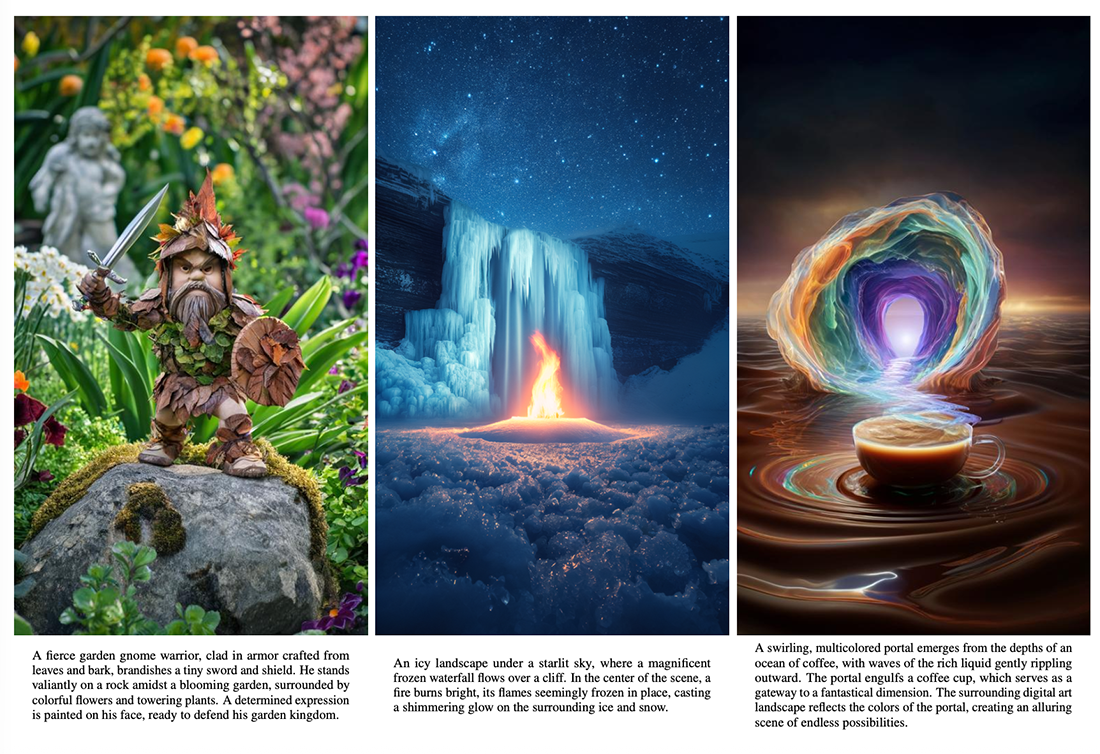
\includegraphics[width=\linewidth]{figures/dalle3.png}};
\begin{scope}[x={(im.south east)},y={(im.north west)}]
\fill[white] (0,0) rectangle (1,.152);
\node[anchor=north west,align=left,inner sep=0pt,text width=.312\linewidth,font=\fontsize{8}{10}\selectfont] at (.018,.145) {一名凶猛的花园侏儒战士，身披用树叶和树皮制成的铠甲，挥舞着一柄小剑和一面小盾。他英勇地站在盛放花园中的岩石上，周围是五颜六色的花朵与高耸的植物。他脸上描绘着坚定的神情，准备保卫自己的花园王国。};
\node[anchor=north west,align=left,inner sep=0pt,text width=.312\linewidth,font=\fontsize{8}{10}\selectfont] at (.347,.145) {星光点点的天空下是一片冰雪景观，一道壮观的冰冻瀑布从悬崖上倾泻而下。场景中央，一团火明亮地燃烧，火苗仿佛凝固在原处，在周围的冰雪上洒下闪烁的光芒。};
\node[anchor=north west,align=left,inner sep=0pt,text width=.312\linewidth,font=\fontsize{8}{10}\selectfont] at (.677,.145) {一个旋转的多彩传送门，从咖啡海洋的深处升起，浓郁液体的波浪轻轻向外荡开。传送门吞没了一杯咖啡，这杯咖啡成为通往奇幻次元的入口。周围的数字艺术景观映照着传送门的色彩，营造出一幅充满无限可能、令人着迷的画面。};
\end{scope}
\end{tikzpicture}

    \caption{DALL-E 3 遵循提示生成图像的示例 \citep{betker2023improving}。}
    \label{fig:dalle3}
\end{figure}

\begin{figure}
    \centering
    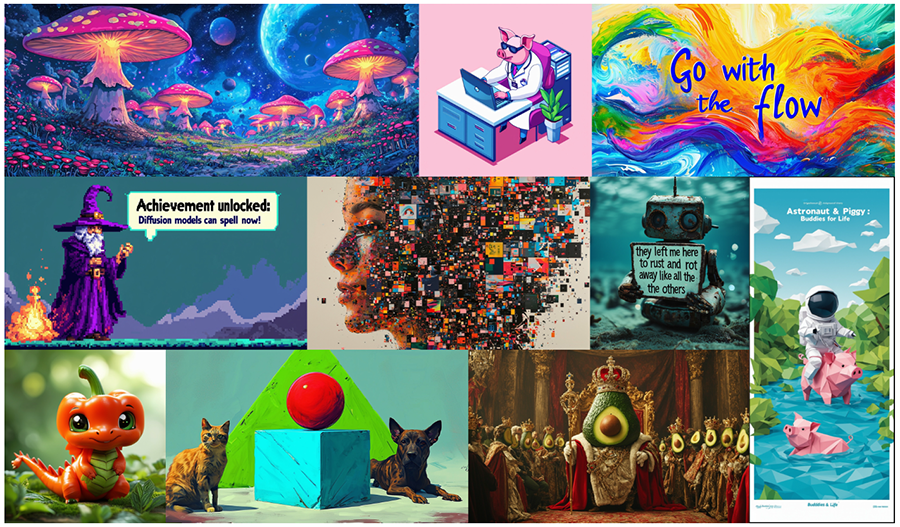
\includegraphics[width=\linewidth]{figures/stablediff}
    \caption{Stable Diffusion 示例 \citep{esser2024scaling}。}
    \label{fig:stablediff}
\end{figure}

\begin{figure}
    \centering
    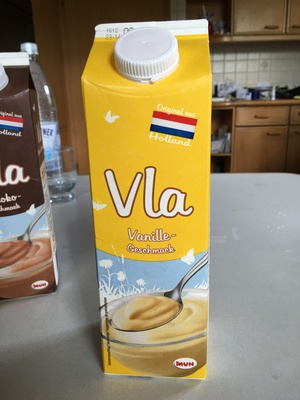
\includegraphics[width=0.4\linewidth]{figures/vla.jpg}\
        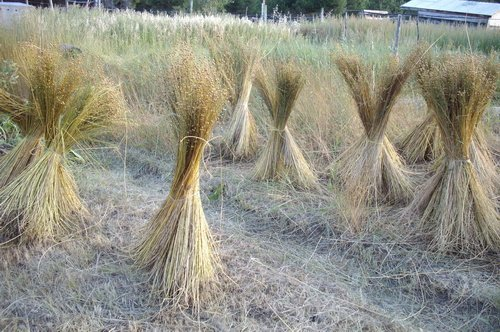
\includegraphics[width=0.4\linewidth]{figures/vlas.jpg}
    \caption{VLA 在不同语言中有不同含义，Vlas 也是如此。图中有一面旗帜，提示了这里使用的是哪种语言。}
    \label{fig:vla}
\end{figure}

\section{决策与视觉语言动作模型}\label{sec:vla}

智能体要行动，就必须决策；要决策，就必须权衡不同选项。本节将介绍如何在状态、动作与奖励构成的回合 $\{(s,a,r)\}$ 上训练 Transformer，另见第~\ref{sec:decisions}~节。这类模型在语言、视觉与机器人动作的序列上训练。视觉语言动作模型，简称 VLA（图~\ref{fig:vla}），经过训练能够输出机器人 API 命令。这是一种特殊的语言：用来引导机器人运动的命令语言。

视觉语言动作模型的任务，是理解视觉场景，并在收到文本命令后，根据摄像头所见，指挥机械臂执行适当动作。这类模型已经取得令人印象深刻的结果，使机器人能够泛化到未见过的情形，成功完成任务。

\begin{figure}
    \centering
    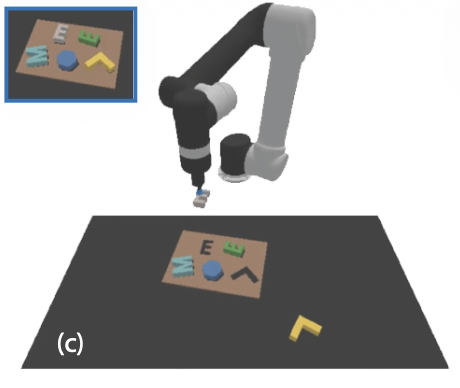
\includegraphics[width=0.5\linewidth]{figures/cliport1}
    \caption{CLIPort 示例：{\em 把灰色字母 E 放进左边 E 形的孔中。}\citep{shridhar2022cliport}}
    \label{fig:cliport1}
\end{figure}

\subsection{任务}
视觉语言动作模型的主要任务，是在现实世界中执行指令，并能够在不断变化的环境中，以具有通用性的方式完成任务。例如，一个机器人操作模型已经学会拾取一组红色铅笔；当任务变为拾取蓝色铅笔时，我们希望模型能够泛化，而不必另行收集包含蓝色铅笔的训练集，再从头训练模型。我们也希望模型能够识别物体，以及物体朝向改变、位置移动或光照变化的情况。模型应当知道如何使用机械臂操作物体、如何执行不同动作。图~\ref{fig:cliport1}~给出了 CLIPort 论文中的一个例子 \citep{shridhar2022cliport}。

\begin{figure}
    \centering
    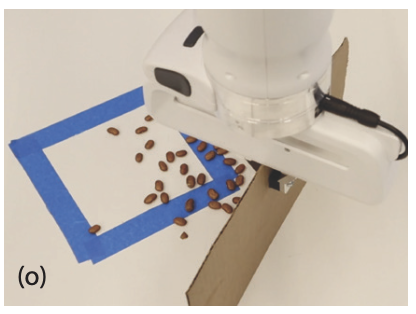
\includegraphics[width=0.5\linewidth]{figures/cliport2}
    \caption{CLIPort 的另一个例子：{\em 把豆子扫进蓝色区域。}\citep{shridhar2020alfworld}}
    \label{fig:cliport2}
\end{figure}

对视觉语言动作模型而言，最困难的任务，是把场景、物体与动作组合成复杂操作，既能处理训练中见过内容的复杂组合，也能泛化到未见过的组合。尤其是在复杂、不断变化、甚至可能是室外的环境中进行长时程导航，是一项艰巨挑战 \citep{shridhar2022cliport}。

在真实的人类与机器人交互情境中，收集更多示范往往不可行。要执行图~\ref{fig:cliport2}~这样的高层任务，模型必须能够识别物体及其位姿，并进行实例分割。模型还必须理解语言，把语言的意义与视觉物体的意义、机器人动作的意义关联起来。

正如下面将看到的，语言为指定目标、跨任务迁移语义概念提供了直观接口。此外，视觉语言模型研究也已经展示了如何从语义层面连接不同类型的嵌入。

\subsection{架构}
了解了任务与挑战后，我们来看看可能采用的模型架构。它们同样可能相当复杂。自然语言方面的结果表明，Transformer 架构非常适合学习序列数据中的模式。直觉上，这意味着它也可能适合对序贯决策问题建模；这类问题通常由用于机器人动作的强化学习方法来解决，第~\ref{sec:sdp}~节已经讨论过，第~\ref{sec:icrl}~节还会进一步深入。在这些问题中，系统从某个状态出发，动作使其进入一个新状态，新状态又有可以采取的动作，如此往复。Transformer 架构很适合对这类问题建模。

决策 Transformer（decision transformer，DT）的早期工作 \citep{chen2021decision,janner2021offline} 表明，在离线、静态的强化学习问题中，GPT 架构确实能够学到最优策略。决策预训练 Transformer（decision-pretrained transformer，DPT）\citet{lee2023supervised,wang2024transformers} 表明，基本 Transformer 架构可以在决策轨迹上预训练与微调。第~\ref{sec:decisions}~节将进一步讨论决策轨迹。

继 CLIPort 的开创性工作之后 \citep{shridhar2022cliport,shridhar2020alfworld}，视觉语言动作模型通常建立在视觉语言模型之上，把机器人命令视为普通语言词元。下面更仔细地考察几种有代表性的模型。

Mobility VLA 的目标是导航 \citep{chiang2024mobility}。它结合长上下文视觉语言模型与拓扑地图构建而成，见图~\ref{fig:mobility}。
\begin{figure}
    \centering
    % 保留原始面板、实拍、示例与全部连线；仅以 TikZ 覆盖说明标签。
\begin{tikzpicture}
\node[anchor=south west,inner sep=0] (im) at (0,0) {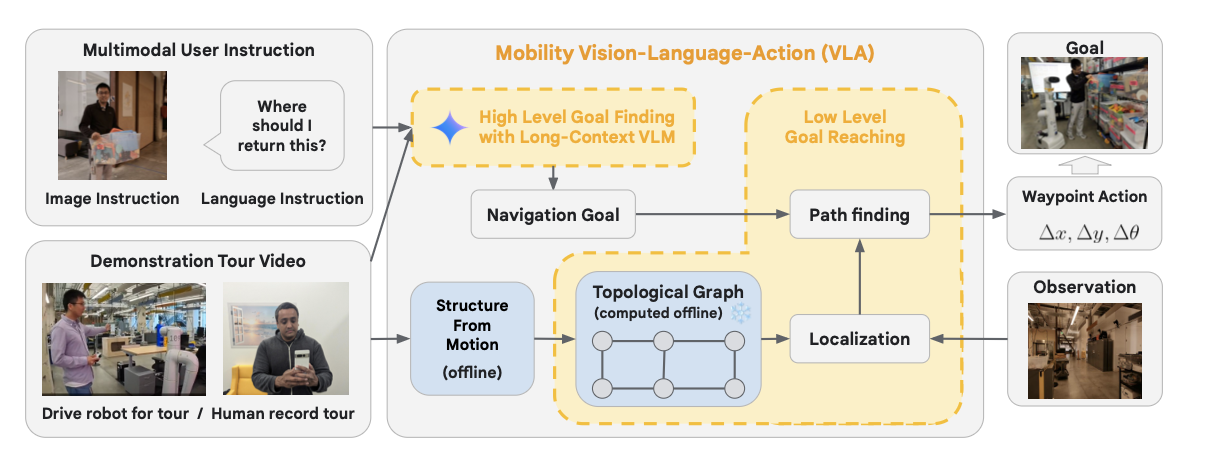
\includegraphics[width=\linewidth]{figures/mobility.png}};
\begin{scope}[x={(im.south east)},y={(im.north west)}]
\fill[white] (0.047855,0.865217) rectangle (0.283828,0.915217);
\node[align=center,inner sep=0pt,font=\fontsize{8.5}{9.5}\selectfont,text width=0.235974\linewidth,rotate=0] at (0.165842,0.890217) {多模态用户指令};
\fill[white] (0.400990,0.854348) rectangle (0.754950,0.915217);
\node[align=center,inner sep=0pt,font=\fontsize{9}{10}\selectfont,text width=0.353960\linewidth,rotate=0] at (0.577970,0.884783) {Mobility 视觉语言动作模型};
\fill[white] (0.858911,0.873913) rectangle (0.936469,0.921739);
\node[align=center,inner sep=0pt,font=\fontsize{8.5}{9.5}\selectfont,text width=0.077558\linewidth,rotate=0] at (0.897690,0.897826) {目标};
\fill[white] (0.191419,0.652174) rectangle (0.276403,0.793478);
\node[align=center,inner sep=0pt,font=\fontsize{8}{9}\selectfont,text width=0.084983\linewidth,rotate=0] at (0.233911,0.722826) {我该把这个\\放回哪里？};
\fill[white] (0.035479,0.539130) rectangle (0.165017,0.584783);
\node[align=center,inner sep=0pt,font=\fontsize{8}{9}\selectfont,text width=0.129538\linewidth,rotate=0] at (0.100248,0.561957) {图像指令};
\fill[white] (0.163366,0.532609) rectangle (0.305281,0.589130);
\node[align=center,inner sep=0pt,font=\fontsize{8}{9}\selectfont,text width=0.127063\linewidth,rotate=0] at (0.241749,0.560870) {语言指令};
\fill[white] (0.050330,0.400000) rectangle (0.274752,0.452174);
\node[align=center,inner sep=0pt,font=\fontsize{8.5}{9.5}\selectfont,text width=0.224422\linewidth,rotate=0] at (0.162541,0.426087) {示范巡视视频};
\fill[white] (0.027228,0.063043) rectangle (0.303630,0.128261);
\node[align=center,inner sep=0pt,font=\fontsize{7.8}{8.8}\selectfont,text width=0.276403\linewidth,rotate=0] at (0.165429,0.095652) {机器人巡视／人工录制巡视};
\fill[white] (0.387789,0.676087) rectangle (0.564356,0.765217);
\node[align=center,inner sep=0pt,font=\fontsize{6.8}{7.8}\selectfont,text width=0.176568\linewidth,rotate=0] at (0.476073,0.720652) {用长上下文视觉语言模型\\寻找高层目标};
\fill[white] (0.400990,0.510870) rectangle (0.512376,0.560870);
\node[align=center,inner sep=0pt,font=\fontsize{8}{9}\selectfont,text width=0.111386\linewidth,rotate=0] at (0.456683,0.535870) {导航目标};
\fill[white] (0.351485,0.158696) rectangle (0.428218,0.363043);
\node[align=center,inner sep=0pt,font=\fontsize{8}{9}\selectfont,text width=0.076733\linewidth,rotate=0] at (0.389851,0.260870) {运动恢复\\结构\\（离线）};
\fill[white] (0.485149,0.291304) rectangle (0.623000,0.384783);
\node[align=center,inner sep=0pt,font=\fontsize{8}{9}\selectfont,text width=0.127888\linewidth,rotate=0] at (0.549092,0.338043) {拓扑图\\（离线计算）};
\fill[white] (0.643000,0.663043) rectangle (0.780000,0.763043);
\node[align=center,inner sep=0pt,font=\fontsize{8}{9}\selectfont,text width=0.125413\linewidth,rotate=0] at (0.712871,0.713043) {底层目标\\到达};
\fill[white] (0.660891,0.506522) rectangle (0.759901,0.563043);
\node[align=center,inner sep=0pt,font=\fontsize{8}{9}\selectfont,text width=0.099010\linewidth,rotate=0] at (0.710396,0.534783) {路径搜索};
\fill[white] (0.655116,0.234783) rectangle (0.761551,0.291304);
\node[align=center,inner sep=0pt,font=\fontsize{8}{9}\selectfont,text width=0.106436\linewidth,rotate=0] at (0.708333,0.263043) {定位};
\fill[white] (0.841584,0.536957) rectangle (0.958746,0.600000);
\node[align=center,inner sep=0pt,font=\fontsize{7.5}{8.5}\selectfont,text width=0.117162\linewidth,rotate=0] at (0.900165,0.568478) {航路点动作};
\fill[white] (0.852310,0.350000) rectangle (0.947195,0.400000);
\node[align=center,inner sep=0pt,font=\fontsize{8}{9}\selectfont,text width=0.094884\linewidth,rotate=0] at (0.899752,0.375000) {观测};
\end{scope}
\end{tikzpicture}

    \caption{Mobility VLA 架构：长上下文视觉语言模型与拓扑地图 \citep{chiang2024mobility}。}
    \label{fig:mobility}
\end{figure}
Mobility VLA 用于一类称为{\em 带示范巡视的多模态指令导航（multi-modal instruction navigation with demonstration tours，MINT）}的导航任务。在这个数据集中，通过预先录制的示范视频提供环境先验。模型采用两层视觉语言动作架构，将长上下文视觉语言模型的环境理解与常识推理，同基于拓扑图的底层导航策略结合起来。高层策略把用户指令与长上下文视觉语言模型结合，在示范视频中找到目标帧。随后，底层策略从这个目标帧出发，遍历拓扑图，在每个时间步生成机器人动作指令。

LM-Nav \citep{shah2023lm} 采用另一种基于现成模型的架构。它的输入包括目标环境的一组原始观测与自由形式的文本指令。模型据此通过三个预训练模型推导行动计划：用语言模型提取地标，用视觉语言模型进行锚定，用视觉导航模型（visual-navigation model，VNM）执行动作，后者与前面介绍的拓扑地图有相似之处。这些模型共同使 LM-Nav 无须任何微调，就能够根据视觉观测遵循文本指令。图~\ref{fig:lmnav}~展示了这一方法。
\begin{figure}
    \centering
    % 保留原始面板、实拍、示例与全部连线；仅以 TikZ 覆盖说明标签。
\begin{tikzpicture}
\node[anchor=south west,inner sep=0] (im) at (0,0) {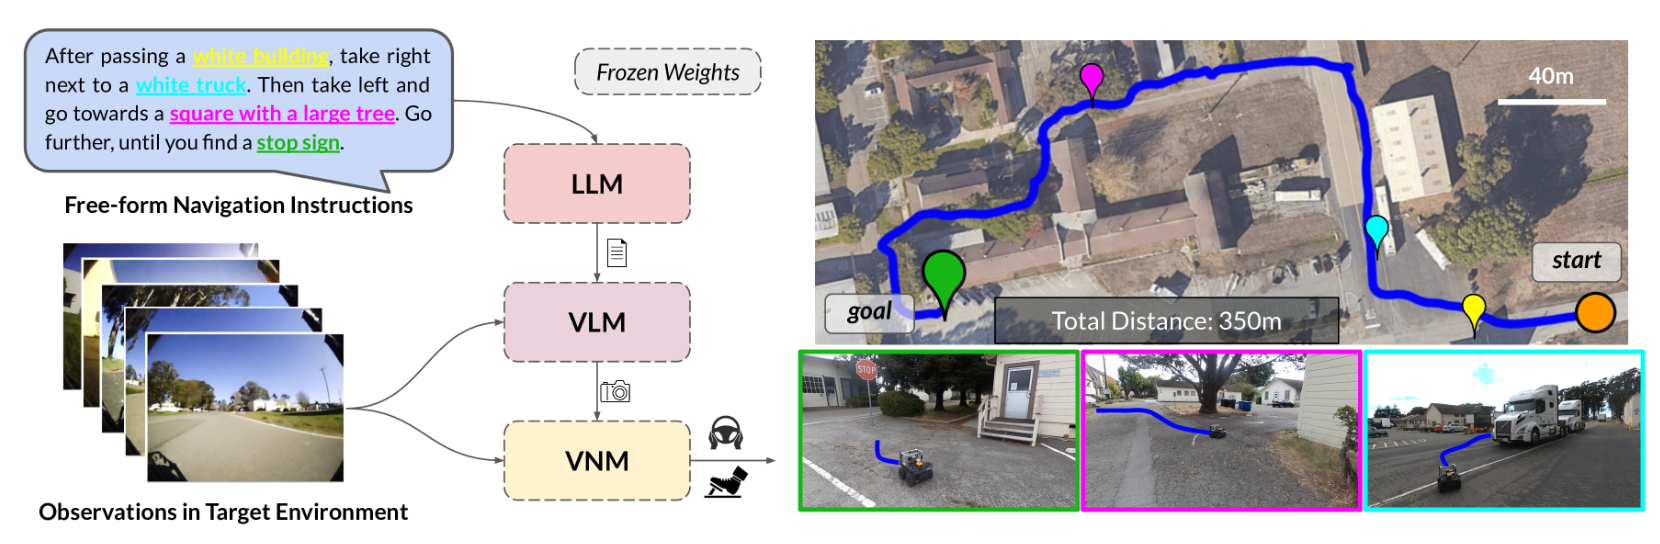
\includegraphics[width=\linewidth]{figures/lmnav.png}};
\begin{scope}[x={(im.south east)},y={(im.north west)}]
\fill[blue!12] (0.022892,0.698529) rectangle (0.266265,0.943015);
\node[align=center,inner sep=0pt,font=\fontsize{7.2}{8.2}\selectfont,text width=0.243373\linewidth,rotate=0] at (0.144578,0.820772) {经过白色建筑后，在白色卡车旁右转。然后左转，前往有大树的广场。继续走，直到找到停止标志。};
\fill[white] (0.031325,0.593750) rectangle (0.259036,0.648897);
\node[align=center,inner sep=0pt,font=\fontsize{8.5}{9.5}\selectfont,text width=0.227711\linewidth,rotate=0] at (0.145181,0.621324) {自由形式导航指令};
\fill[white] (0.351807,0.840074) rectangle (0.454217,0.904412);
\node[align=center,inner sep=0pt,font=\fontsize{8}{9}\selectfont,text width=0.102410\linewidth,rotate=0] at (0.403012,0.872243) {冻结权重};
\fill[white] (0.017470,0.022059) rectangle (0.266265,0.082721);
\node[align=center,inner sep=0pt,font=\fontsize{8.5}{9.5}\selectfont,text width=0.248795\linewidth,rotate=0] at (0.141867,0.052390) {目标环境中的观测};
\fill[gray!30] (0.602410,0.380515) rectangle (0.802410,0.448529);
\node[align=center,inner sep=0pt,font=\fontsize{8.5}{9.5}\selectfont,text width=0.200000\linewidth,rotate=0] at (0.702410,0.414522) {总距离：350 米};
\fill[gray!15] (0.928313,0.487132) rectangle (0.973494,0.544118);
\node[align=center,inner sep=0pt,font=\fontsize{8}{9}\selectfont,text width=0.045181\linewidth,rotate=0] at (0.950904,0.515625) {起点};
\fill[gray!15] (0.500000,0.391544) rectangle (0.542169,0.452206);
\node[align=center,inner sep=0pt,font=\fontsize{8}{9}\selectfont,text width=0.042169\linewidth,rotate=0] at (0.521084,0.421875) {终点};
\end{scope}
\end{tikzpicture}

    \caption{LM-Nav 的三大语言模型架构 \citep{shah2023lm}。}
    \label{fig:lmnav}
\end{figure}

Google 的 RT-2 \citep{brohan2023rt} 采用不同方法，其思想是利用网络知识指导机器人控制：让机器人通过观看视频，学习如何行动。标准视觉语言模型同时在文本形式的机器人轨迹数据，以及互联网规模的视觉语言任务（例如视觉问答）上微调。机器人动作表示为普通文本词元，与自然语言词元一样，直接纳入训练集，见图~\ref{fig:rt2}。
\begin{figure}
    \centering
    % 保留原始面板、实拍、示例与全部连线；仅以 TikZ 覆盖说明标签。
\begin{tikzpicture}
\node[anchor=south west,inner sep=0] (im) at (0,0) {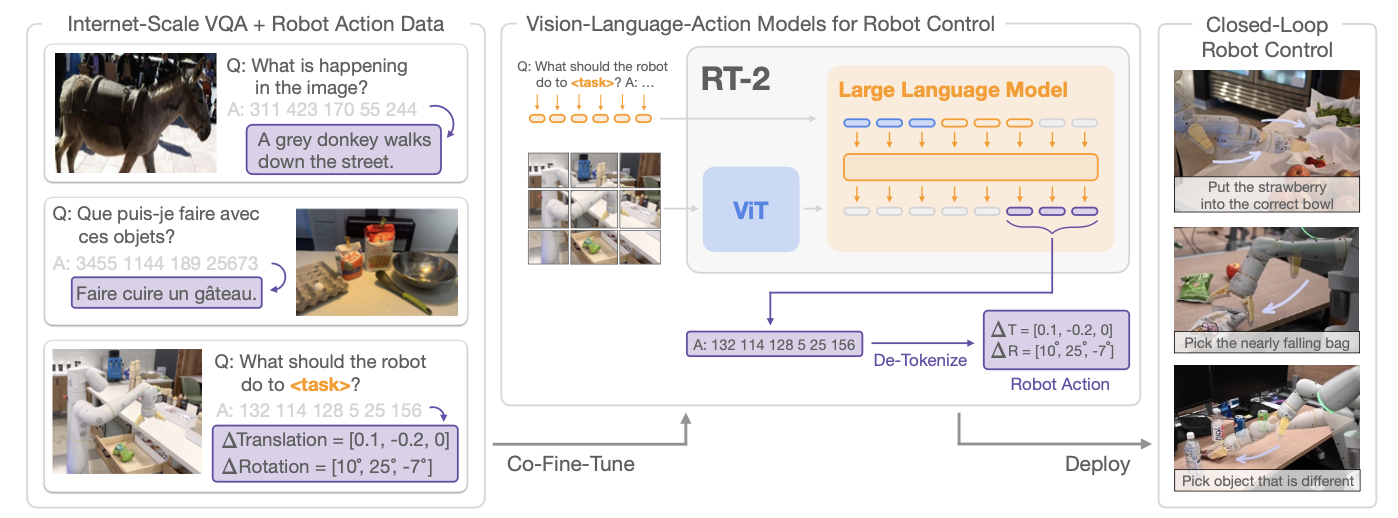
\includegraphics[width=\linewidth]{figures/rt2.png}};
\begin{scope}[x={(im.south east)},y={(im.north west)}]
\fill[white] (0.043634,0.930502) rectangle (0.317597,0.980695);
\node[align=center,inner sep=0pt,font=\fontsize{7.5}{8.5}\selectfont,text width=0.273963\linewidth,rotate=0] at (0.180615,0.955598) {互联网级 VQA 与机器人动作数据};
\fill[white] (0.371960,0.930502) rectangle (0.806152,0.978764);
\node[align=center,inner sep=0pt,font=\fontsize{8.5}{9.5}\selectfont,text width=0.434192\linewidth,rotate=0] at (0.589056,0.954633) {用于机器人控制的视觉语言动作模型};
\fill[white] (0.854077,0.874517) rectangle (0.968526,0.978764);
\node[align=center,inner sep=0pt,font=\fontsize{8.5}{9.5}\selectfont,text width=0.114449\linewidth,rotate=0] at (0.911302,0.926641) {闭环\\机器人控制};
\fill[orange!10] (0.596567,0.797297) rectangle (0.790415,0.849421);
\node[align=center,inner sep=0pt,font=\fontsize{9}{10}\selectfont,text width=0.193848\linewidth,rotate=0] at (0.693491,0.823359) {大语言模型};
\fill[white] (0.620172,0.281853) rectangle (0.697425,0.322394);
\node[align=center,inner sep=0pt,font=\fontsize{7.5}{8.5}\selectfont,text width=0.077253\linewidth,rotate=0] at (0.658798,0.302124) {反词元化};
\fill[white] (0.713162,0.223938) rectangle (0.800429,0.270270);
\node[align=center,inner sep=0pt,font=\fontsize{7.5}{8.5}\selectfont,text width=0.087268\linewidth,rotate=0] at (0.756795,0.247104) {机器人动作};
\fill[white] (0.360515,0.077220) rectangle (0.469957,0.129344);
\node[align=center,inner sep=0pt,font=\fontsize{8.5}{9.5}\selectfont,text width=0.109442\linewidth,rotate=0] at (0.415236,0.103282) {联合微调};
\fill[white] (0.756795,0.075290) rectangle (0.827611,0.135135);
\node[align=center,inner sep=0pt,font=\fontsize{8.5}{9.5}\selectfont,text width=0.070815\linewidth,rotate=0] at (0.792203,0.105212) {部署};
\fill[gray!15] (0.842632,0.590734) rectangle (0.972818,0.658301);
\node[align=center,inner sep=0pt,font=\fontsize{6.5}{7.5}\selectfont,text width=0.130186\linewidth,rotate=0] at (0.907725,0.624517) {草莓放入正确的碗中};
\fill[gray!15] (0.842632,0.050193) rectangle (0.973534,0.100386);
\node[align=center,inner sep=0pt,font=\fontsize{6.5}{7.5}\selectfont,text width=0.130901\linewidth,rotate=0] at (0.908083,0.075290) {挑出不同的物体};
% 完整中文化问答示例；数值词元、占位符、照片与连线保持原样。
\fill[white] (0.158798,0.808880) rectangle (0.317597,0.895753);
\node[anchor=north west,align=left,inner sep=0pt,font=\fontsize{6.2}{7.1}\selectfont,text width=0.155937\linewidth] at (0.160229,0.891892) {问：图像中发生了什么？};
\fill[violet!14] (0.178112,0.669884) rectangle (0.313305,0.752896);
\node[anchor=center,align=center,inner sep=0pt,font=\fontsize{6.2}{7.1}\selectfont,text width=0.132332\linewidth] at (0.245708,0.711390) {一头灰驴走在街上。};
\fill[white] (0.035765,0.517375) rectangle (0.209585,0.604247);
\node[anchor=north west,align=left,inner sep=0pt,font=\fontsize{6.2}{7.1}\selectfont,text width=0.170959\linewidth] at (0.037196,0.600386) {问：这些东西能做什么？};
\fill[violet!14] (0.053648,0.415058) rectangle (0.185980,0.459459);
\node[anchor=center,align=center,inner sep=0pt,font=\fontsize{6.2}{7.1}\selectfont,text width=0.129471\linewidth] at (0.119814,0.437259) {烤一个蛋糕。};
\fill[white] (0.153076,0.229730) rectangle (0.319742,0.322394);
\node[anchor=north west,align=left,inner sep=0pt,font=\fontsize{6.2}{7.1}\selectfont,text width=0.163805\linewidth] at (0.154506,0.318533) {问：机器人如何完成\texttt{<task>}？};
\fill[violet!14] (0.154506,0.077220) rectangle (0.324034,0.171815);
\node[anchor=center,align=center,inner sep=0pt,font=\fontsize{6.0}{7.2}\selectfont,text width=0.166667\linewidth] at (0.239270,0.124517) {$\Delta\text{平移}=[0.1,-0.2,0]$\\$\Delta\text{旋转}=[10^\circ,25^\circ,-7^\circ]$};
\fill[white] (0.367668,0.820463) rectangle (0.479971,0.895753);
\node[anchor=north west,align=left,inner sep=0pt,font=\fontsize{4.8}{5.4}\selectfont,text width=0.109442\linewidth] at (0.369099,0.891892) {问：机器人如何\\完成\texttt{<task>}？答：…};
\fill[gray!15] (0.840486,0.590734) rectangle (0.975680,0.656371);
\node[anchor=center,align=center,inner sep=0pt,font=\fontsize{6.0}{6.8}\selectfont,text width=0.132332\linewidth] at (0.908083,0.623552) {把草莓放入正确的碗中};
\fill[gray!15] (0.841917,0.322394) rectangle (0.970672,0.357143);
\node[anchor=center,align=center,inner sep=0pt,font=\fontsize{6.0}{6.8}\selectfont,text width=0.125894\linewidth] at (0.906295,0.339768) {拿起即将掉落的袋子};
\end{scope}
\end{tikzpicture}

    \caption{RT-2 架构：把机器人动作作为文本词元训练的视觉语言模型 \citep{brohan2023rt}。}
    \label{fig:rt2}
\end{figure}
Magma \citep{yang2025magma} 采用相似方法，在涵盖图像、视频与机器人数据的异构数据集上预训练。不过，Magma 使用特殊词元标记图像中可交互的视觉物体，即标记集合（Set-of-Mark），以实现动作锚定。类似地，物体运动，例如人手或机械臂的轨迹，通过标记轨迹（Trace-of-Mark）表示，以便进行动作规划。图~\ref{fig:magma}~给出了示意。
\begin{figure}
    \centering
    % 保留原始面板、实拍、示例与全部连线；仅以 TikZ 覆盖说明标签。
\begin{tikzpicture}
\node[anchor=south west,inner sep=0] (im) at (0,0) {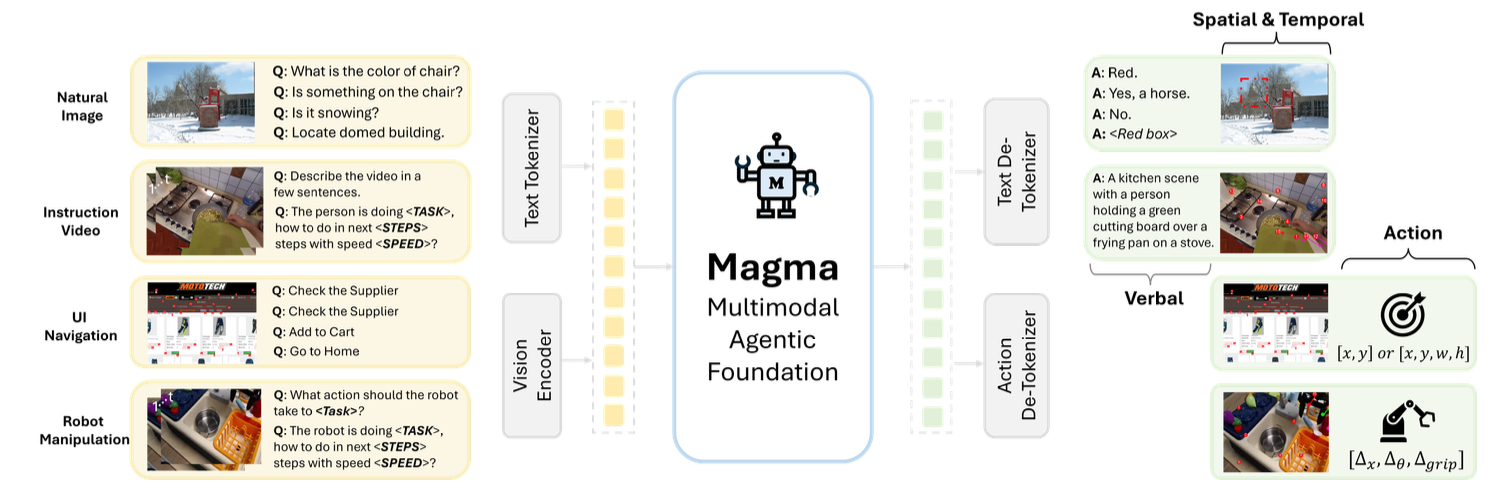
\includegraphics[width=\linewidth]{figures/magma.png}};
\begin{scope}[x={(im.south east)},y={(im.north west)}]
\fill[white] (0.029570,0.743902) rectangle (0.081989,0.821138);
\node[align=center,inner sep=0pt,font=\fontsize{8}{9}\selectfont,text width=0.052419\linewidth,rotate=0] at (0.055780,0.782520) {自然图像};
\fill[white] (0.025538,0.506098) rectangle (0.081989,0.587398);
\node[align=center,inner sep=0pt,font=\fontsize{8}{9}\selectfont,text width=0.056452\linewidth,rotate=0] at (0.053763,0.546748) {指令视频};
\fill[white] (0.026882,0.296748) rectangle (0.081317,0.376016);
\node[align=center,inner sep=0pt,font=\fontsize{8}{9}\selectfont,text width=0.054435\linewidth,rotate=0] at (0.054099,0.336382) {界面导航};
\fill[white] (0.023522,0.048780) rectangle (0.087366,0.191057);
\node[align=center,inner sep=0pt,font=\fontsize{7.5}{8.5}\selectfont,text width=0.063844\linewidth,rotate=0] at (0.055444,0.119919) {机器人\\操作};
\fill[white] (0.338710,0.510163) rectangle (0.372312,0.788618);
\node[align=center,inner sep=0pt,font=\fontsize{7.5}{8.5}\selectfont,text width=0.033602\linewidth,rotate=0] at (0.355511,0.649390) {文本\\词元化器};
\fill[white] (0.338710,0.123984) rectangle (0.373656,0.392276);
\node[align=center,inner sep=0pt,font=\fontsize{7.5}{8.5}\selectfont,text width=0.034946\linewidth,rotate=0] at (0.356183,0.258130) {视觉\\编码器};
\fill[white] (0.460349,0.193089) rectangle (0.580645,0.410569);
\node[align=center,inner sep=0pt,font=\fontsize{9}{10}\selectfont,text width=0.120296\linewidth,rotate=0] at (0.520497,0.301829) {多模态\\智能体\\基础模型};
\fill[white] (0.661962,0.512195) rectangle (0.702285,0.792683);
\node[align=center,inner sep=0pt,font=\fontsize{7.5}{8.5}\selectfont,text width=0.040323\linewidth,rotate=0] at (0.682124,0.652439) {文本反\\词元化器};
\fill[white] (0.663306,0.121951) rectangle (0.701613,0.384146);
\node[align=center,inner sep=0pt,font=\fontsize{7.5}{8.5}\selectfont,text width=0.038306\linewidth,rotate=0] at (0.682460,0.253049) {动作反\\词元化器};
\fill[white] (0.797043,0.932927) rectangle (0.927419,0.985772);
\node[align=center,inner sep=0pt,font=\fontsize{8.5}{9.5}\selectfont,text width=0.130376\linewidth,rotate=0] at (0.862231,0.959350) {空间与时间};
\fill[white] (0.749328,0.367886) rectangle (0.805108,0.416667);
\node[align=center,inner sep=0pt,font=\fontsize{8.5}{9.5}\selectfont,text width=0.055780\linewidth,rotate=0] at (0.777218,0.392276) {语言};
\fill[white] (0.927419,0.502033) rectangle (0.979839,0.550813);
\node[align=center,inner sep=0pt,font=\fontsize{8.5}{9.5}\selectfont,text width=0.052419\linewidth,rotate=0] at (0.953629,0.526423) {动作};
% 完整中文化问答示例；数值词元、占位符、照片与连线保持原样。
\fill[yellow!9] (0.181452,0.709350) rectangle (0.312500,0.873984);
\node[anchor=north west,align=left,inner sep=0pt,font=\fontsize{4.8}{5.4}\selectfont,text width=0.128360\linewidth] at (0.182796,0.869919) {问：椅子是什么颜色？\\问：椅子上有东西吗？\\问：在下雪吗？\\问：定位圆顶建筑。};
\fill[yellow!9] (0.181452,0.483740) rectangle (0.312500,0.652439);
\node[anchor=north west,align=left,inner sep=0pt,font=\fontsize{5.0}{5.8}\selectfont,text width=0.128360\linewidth] at (0.182796,0.648374) {问：用几句话描述视频。\\问：此人正做\texttt{<TASK>}；\\接下来如何以\texttt{<SPEED>}\\速度完成\texttt{<STEPS>}步？};
\fill[yellow!9] (0.181452,0.270325) rectangle (0.312500,0.426829);
\node[anchor=north west,align=left,inner sep=0pt,font=\fontsize{5.0}{5.4}\selectfont,text width=0.128360\linewidth] at (0.182796,0.422764) {问：查看供应商\\问：查看供应商\\问：加入购物车\\问：回到首页};
\fill[yellow!9] (0.181452,0.034553) rectangle (0.312500,0.223577);
\node[anchor=north west,align=left,inner sep=0pt,font=\fontsize{4.6}{5.0}\selectfont,text width=0.128360\linewidth] at (0.182796,0.219512) {问：机器人应如何\\完成\texttt{<Task>}？\\问：机器人正做\texttt{<TASK>}；\\接下来如何以\texttt{<SPEED>}\\速度完成\texttt{<STEPS>}步？};
\fill[green!6] (0.731855,0.709350) rectangle (0.817204,0.873984);
\node[anchor=north west,align=left,inner sep=0pt,font=\fontsize{4.6}{5.1}\selectfont,text width=0.082661\linewidth] at (0.733199,0.869919) {答：红色。\\答：是，一匹马\\答：没有。\\答：\texttt{<Red box>}};
\fill[green!6] (0.731855,0.483740) rectangle (0.817876,0.654472);
\node[anchor=north west,align=left,inner sep=0pt,font=\fontsize{5.0}{5.5}\selectfont,text width=0.083333\linewidth] at (0.733199,0.650407) {答：厨房中，一人手持绿色切菜板，悬在灶台上的煎锅上方。};
\end{scope}
\end{tikzpicture}

    \caption{Magma 预训练流程 \citep{yang2025magma}。}
    \label{fig:magma}
\end{figure}

最后，名为 $\pi_0$ 的视觉语言动作模型 \citep{black2024pi_0} 强调强化学习方法，采用预训练的后期融合视觉语言模型，以及包含多种操作任务的多样化跨具身数据集。该模型受到 Transfusion 方法启发 \citep{zhou2024transfusion}，通过增加一个独立的动作专家（action expert）来适应机器人控制。动作专家通过流匹配（flow matching）产生动作，实现流畅的操作技能。最终模型既可以直接根据提示执行任务，也可以在更高质量数据上进一步微调，从而完成复杂的多阶段任务，例如折叠多件衣物或组装盒子，见图~\ref{fig:pizero}。
\begin{figure}
    \centering
    % 保留原始面板、实拍、示例与全部连线；仅以 TikZ 覆盖说明标签。
\begin{tikzpicture}
\node[anchor=south west,inner sep=0] (im) at (0,0) {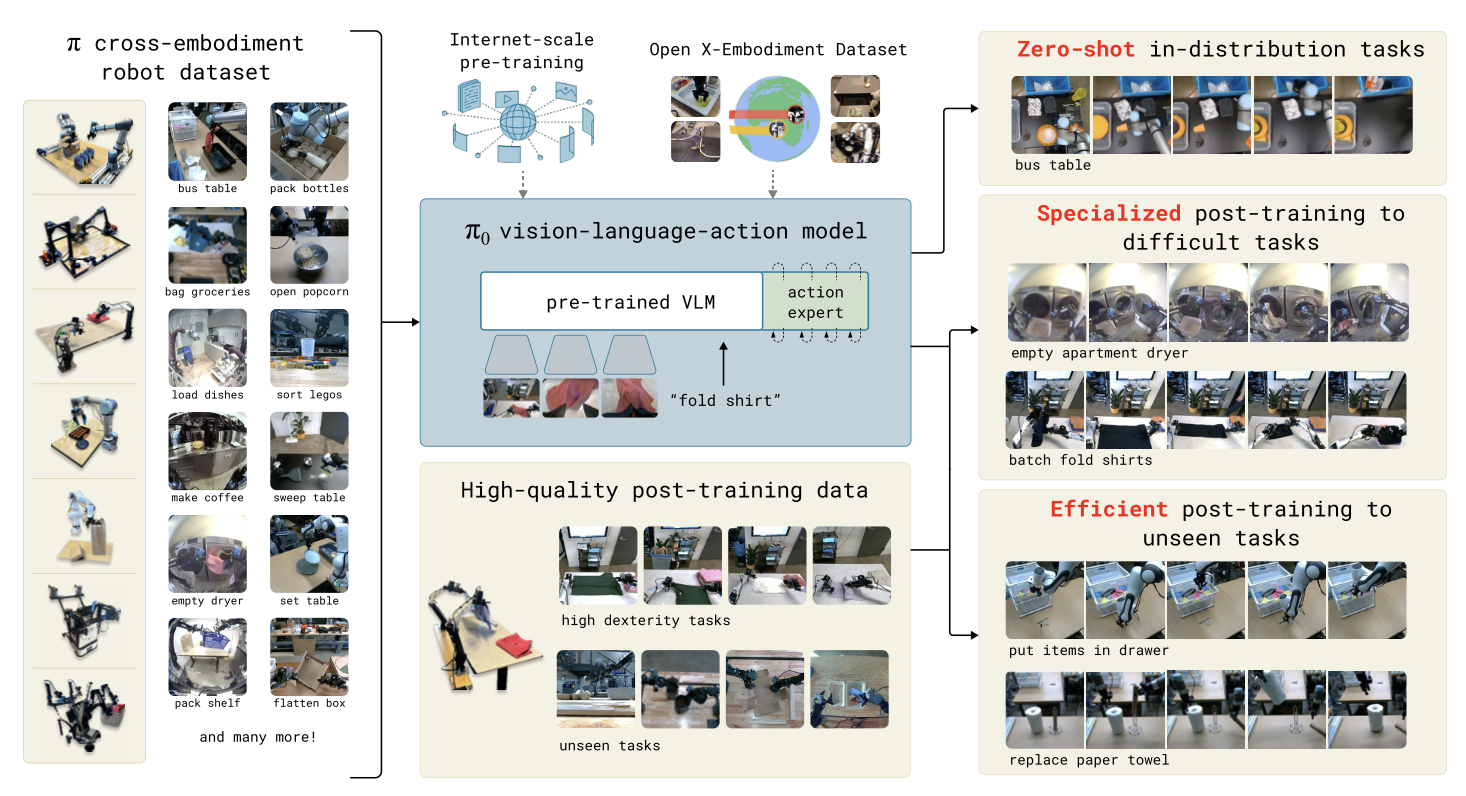
\includegraphics[width=\linewidth]{figures/pizero.png}};
\begin{scope}[x={(im.south east)},y={(im.north west)}]
\fill[white] (0.045703,0.896985) rectangle (0.223056,0.964824);
\node[align=center,inner sep=0pt,font=\fontsize{9}{10}\selectfont,text width=0.177353\linewidth,rotate=0] at (0.134379,0.930905) {$\pi$ 跨具身\\机器人数据集};
\fill[white] (0.304911,0.907035) rectangle (0.415416,0.966080);
\node[align=center,inner sep=0pt,font=\fontsize{8}{9}\selectfont,text width=0.110505\linewidth,rotate=0] at (0.360164,0.936558) {互联网规模\\预训练};
\fill[white] (0.440655,0.922111) rectangle (0.622101,0.954774);
\node[align=center,inner sep=0pt,font=\fontsize{8}{9}\selectfont,text width=0.181446\linewidth,rotate=0] at (0.531378,0.938442) {Open X-Embodiment 数据集};
\fill[blue!12] (0.314461,0.689698) rectangle (0.596180,0.728643);
\node[align=center,inner sep=0pt,font=\fontsize{9}{10}\selectfont,text width=0.281719\linewidth,rotate=0] at (0.455321,0.709171) {$\pi_0$ 视觉语言动作模型};
\fill[white] (0.331514,0.587940) rectangle (0.516371,0.655779);
\node[align=center,inner sep=0pt,font=\fontsize{8}{9}\selectfont,text width=0.184857\linewidth,rotate=0] at (0.423943,0.621859) {预训练视觉语言模型};
\fill[green!15] (0.524557,0.587940) rectangle (0.590723,0.655779);
\node[align=center,inner sep=0pt,font=\fontsize{7.2}{8.2}\selectfont,text width=0.066166\linewidth,rotate=0] at (0.557640,0.621859) {动作\\专家};
\fill[blue!12] (0.452251,0.476131) rectangle (0.553206,0.512563);
\node[align=center,inner sep=0pt,font=\fontsize{7.2}{8.2}\selectfont,text width=0.100955\linewidth,rotate=0] at (0.502729,0.494347) {“折叠衬衫”};
\fill[white] (0.309686,0.365578) rectangle (0.607776,0.402010);
\node[align=center,inner sep=0pt,font=\fontsize{9}{10}\selectfont,text width=0.298090\linewidth,rotate=0] at (0.458731,0.383794) {高质量后训练数据};
\fill[white] (0.384038,0.201005) rectangle (0.584584,0.231156);
\node[align=center,inner sep=0pt,font=\fontsize{8}{9}\selectfont,text width=0.200546\linewidth,rotate=0] at (0.484311,0.216080) {高灵巧度任务};
\fill[white] (0.379945,0.047739) rectangle (0.513643,0.075377);
\node[align=center,inner sep=0pt,font=\fontsize{8}{9}\selectfont,text width=0.133697\linewidth,rotate=0] at (0.446794,0.061558) {未见过的任务};
\fill[white] (0.687585,0.920854) rectangle (0.979536,0.953518);
\node[align=center,inner sep=0pt,font=\fontsize{9}{10}\selectfont,text width=0.291951\linewidth,rotate=0] at (0.833561,0.937186) {分布内任务的零样本表现};
\fill[white] (0.703274,0.776382) rectangle (0.772851,0.802764);
\node[align=center,inner sep=0pt,font=\fontsize{7.5}{8.5}\selectfont,text width=0.069577\linewidth,rotate=0] at (0.738063,0.789573) {收拾餐桌};
\fill[white] (0.685539,0.683417) rectangle (0.980900,0.747487);
\node[align=center,inner sep=0pt,font=\fontsize{9}{10}\selectfont,text width=0.295362\linewidth,rotate=0] at (0.833220,0.715452) {通过专门后训练\\完成困难任务};
\fill[white] (0.688267,0.542714) rectangle (0.843111,0.567839);
\node[align=center,inner sep=0pt,font=\fontsize{7.5}{8.5}\selectfont,text width=0.154843\linewidth,rotate=0] at (0.765689,0.555276) {清空公寓中的烘干机};
\fill[white] (0.685539,0.407035) rectangle (0.850614,0.434673);
\node[align=center,inner sep=0pt,font=\fontsize{7.5}{8.5}\selectfont,text width=0.165075\linewidth,rotate=0] at (0.768076,0.420854) {批量折叠衬衫};
\fill[white] (0.684857,0.309045) rectangle (0.978854,0.374372);
\node[align=center,inner sep=0pt,font=\fontsize{9}{10}\selectfont,text width=0.293997\linewidth,rotate=0] at (0.831855,0.341709) {通过高效后训练\\完成未见过的任务};
\fill[white] (0.685539,0.163317) rectangle (0.850614,0.193467);
\node[align=center,inner sep=0pt,font=\fontsize{7.5}{8.5}\selectfont,text width=0.165075\linewidth,rotate=0] at (0.768076,0.178392) {把物品放入抽屉};
\fill[white] (0.685539,0.026382) rectangle (0.854025,0.055276);
\node[align=center,inner sep=0pt,font=\fontsize{7.5}{8.5}\selectfont,text width=0.168486\linewidth,rotate=0] at (0.769782,0.040829) {更换厨房纸卷};
\fill[white] (0.131651,0.057789) rectangle (0.228513,0.085427);
\node[align=center,inner sep=0pt,font=\fontsize{8}{9}\selectfont,text width=0.096862\linewidth,rotate=0] at (0.180082,0.071608) {还有更多！};
\fill[white] (0.107776,0.747487) rectangle (0.173943,0.776382);
\node[align=center,inner sep=0pt,font=\fontsize{6.2}{7.2}\selectfont,text width=0.066166\linewidth,rotate=0] at (0.140859,0.761935) {收餐桌};
\fill[white] (0.177353,0.747487) rectangle (0.243520,0.776382);
\node[align=center,inner sep=0pt,font=\fontsize{6.2}{7.2}\selectfont,text width=0.066166\linewidth,rotate=0] at (0.210437,0.761935) {装瓶};
\fill[white] (0.107776,0.615578) rectangle (0.173943,0.644472);
\node[align=center,inner sep=0pt,font=\fontsize{6.2}{7.2}\selectfont,text width=0.066166\linewidth,rotate=0] at (0.140859,0.630025) {杂货装袋};
\fill[white] (0.177353,0.615578) rectangle (0.243520,0.644472);
\node[align=center,inner sep=0pt,font=\fontsize{6.2}{7.2}\selectfont,text width=0.066166\linewidth,rotate=0] at (0.210437,0.630025) {开爆米花};
\fill[white] (0.107776,0.483668) rectangle (0.173943,0.512563);
\node[align=center,inner sep=0pt,font=\fontsize{6.2}{7.2}\selectfont,text width=0.066166\linewidth,rotate=0] at (0.140859,0.498116) {装餐具};
\fill[white] (0.177353,0.483668) rectangle (0.243520,0.512563);
\node[align=center,inner sep=0pt,font=\fontsize{6.2}{7.2}\selectfont,text width=0.066166\linewidth,rotate=0] at (0.210437,0.498116) {理乐高};
\fill[white] (0.107776,0.351759) rectangle (0.173943,0.380653);
\node[align=center,inner sep=0pt,font=\fontsize{6.2}{7.2}\selectfont,text width=0.066166\linewidth,rotate=0] at (0.140859,0.366206) {煮咖啡};
\fill[white] (0.177353,0.351759) rectangle (0.243520,0.380653);
\node[align=center,inner sep=0pt,font=\fontsize{6.2}{7.2}\selectfont,text width=0.066166\linewidth,rotate=0] at (0.210437,0.366206) {扫桌面};
\fill[white] (0.107776,0.221106) rectangle (0.173943,0.250000);
\node[align=center,inner sep=0pt,font=\fontsize{6.2}{7.2}\selectfont,text width=0.066166\linewidth,rotate=0] at (0.140859,0.235553) {清烘干机};
\fill[white] (0.177353,0.221106) rectangle (0.243520,0.250000);
\node[align=center,inner sep=0pt,font=\fontsize{6.2}{7.2}\selectfont,text width=0.066166\linewidth,rotate=0] at (0.210437,0.235553) {摆餐桌};
\fill[white] (0.107776,0.089196) rectangle (0.173943,0.118090);
\node[align=center,inner sep=0pt,font=\fontsize{6.2}{7.2}\selectfont,text width=0.066166\linewidth,rotate=0] at (0.140859,0.103643) {整理货架};
\fill[white] (0.177353,0.089196) rectangle (0.243520,0.118090);
\node[align=center,inner sep=0pt,font=\fontsize{6.2}{7.2}\selectfont,text width=0.066166\linewidth,rotate=0] at (0.210437,0.103643) {压平盒子};
\end{scope}
\end{tikzpicture}

    \caption{$\pi_0$ 架构。该模型基于视觉语言模型，并由跨具身数据集加以增强 \citep{black2024pi_0}。}
    \label{fig:pizero}
\end{figure}

\subsection{学习算法}
大多数视觉语言动作模型的架构建立在视觉语言模型之上，有时还加入导航地图数据。机器人动作命令通常编码为普通文本命令。与视觉语言模型及决策 Transformer 相似，预训练与微调也采用典型的大语言模型自监督学习算法。有时，为了减少训练成本，会使用现成的预训练模型。

\subsection{结果}
已经出现多种视觉语言动作模型，取得了令人印象深刻的零样本结果，使行为能够泛化到未见过的情形。\citet{chiang2024mobility,brohan2023rt,yang2025magma} 提供了机器人动作模型的例子，能够完成导航、桌面操作，甚至折叠衣物等复杂任务 \citep{black2024pi_0}。

视觉语言动作模型取得了出色且富有想象力的结果，使机器人在推理阶段无须重新训练，就能够泛化。有关这类模型的综述，参见 \citep{ma2024survey}。

观看视频最能体会这些结果。$\pi_0$ 有展示视频，\footnote{\url{https://www.physicalintelligence.company/blog/pi0}}RT-2 也有展示视频。\footnote{\url{https://robotics-transformer2.github.io}}

\section{世界模型、物理与规划}\label{sec:world}

对视觉语言模型而言，图像由像素组成，本身并不带有更深的内在意义。不过，与世界交互的智能体需要了解世界的物理属性。模型必须理解哪些事情在物理上可能发生，使智能体不至于像电子游戏中有时仍会出现的那样，穿墙而过。

世界模型帮助智能体理解世界，使其能够在物理世界中有效行动，采取合理的动作。大语言模型最初是语言模型。我们能够用自然语言与它们交谈，它们也必然包含一些世界知识，但并未专门接受训练，以便广泛、深入地理解世间事物。一些研究者认为，为了让智能体大语言模型真正取得成功，并使大语言模型达到较高的通用智能水平，应当加强世界模型研究 \citep{sutton2022alberta,matsuo2022deep,lecun2022path,klindt2026does}。

在世界中行动的智能体与机器人，需要对世界的物理规律有初步理解。训练大语言模型的一项挑战，是将其对物理世界与可行机器人动作的理解锚定于现实。一种办法，是根据动作反馈，学习一个关于世界，也就是环境的智能体模型。

{\em 世界模型}一词在人工智能的其他语境中也曾使用。最值得注意的是，它指基于模型的强化学习中的{\em 模型} \citep{ha2018world,moerland2023model,sutton1991dyna}，见下一小节。这个模型根据智能体与环境的交互，保存关于环境的一部分知识的本地副本，用以改进行动策略。世界模型包含一种通过学习获得的、高效而压缩的世界表示 \citep{hafner2018learning,plaat2020deep}。这类表示通常称为抽象表示或{\em 潜在（latent）}表示，以区别于环境中真实世界的常规表示。世界模型通常经过训练，掌握物理规律与某些空间属性的知识，由此约束智能体的动作。世界模型的具体内容，取决于智能体所在的领域。

需要注意，短短几章之间，我们已经从理解语言，走到了理解世界。大型{\em 语言}模型的目标，是从文本的统计模式中理解自然语言的某些语义，用于问答与翻译；{\em 世界}模型的目标，则是理解物理规律中的因果关系，用来为智能体模拟未来的世界状态。从大语言模型走向智能体大语言模型，需要相当多的新技术。

先来看看世界模型目前如何用于智能体大语言模型。

\subsection{任务}
世界模型应当封装世界知识，使智能体能够执行有意义的动作。这些动作应当锚定于物理世界。例如，模型应当理解受其控制的机械臂关节有哪些限制；导航智能体应当理解重力、距离以及墙壁是实体等物理概念；金融智能体应当理解银行账户余额为负的后果。这类信息通常是人类习以为常的常识，因此，当智能体不能理解其所在世界的这些基本事实时，我们会感到惊讶。只在像素上训练的视觉语言模型，可能无法把握特定纹理的语义，不知道它究竟是衣物、烟雾，还是墙壁。

标准预训练大语言模型已经包含一些有用的世界知识。它们通过基于人类反馈的强化学习，学会可接受的文本行为；通过可验证奖励强化学习，学会可接受的数学与编程行为。一些早期方法把大语言模型直接用作预训练世界模型，无须任何微调。学习世界物理规律的一种自然方式，是交互：智能体可以通过类似强化学习的奖励函数，学会可接受的物理行为。

在基于模型的强化学习中，世界模型的目标，是通过在世界{\em 模型}中规划，而不是从{\em 真实}世界采样，提高交互学习的样本效率。当与世界交互比执行模拟更昂贵时，这一点尤其有用，智能体大语言模型中往往如此。下面介绍的大语言模型世界模型方法，使用了基于模型的强化学习技术，见第~\ref{sec:mbrl}~节。目前，大语言模型中的世界模型方法相当多样。为了说明它们用于哪些任务，我们将讨论三个例子：WorldGPT、WebDreamer 与 WorldCoder。

\paragraph{WorldGPT}
WorldGPT \citep{ge2024worldgpt} 的目标，是解决视觉问答与具身规划任务，包括音视频问答。WorldGPT 从视频中学习一个世界视觉语言模型，采用潜在空间视觉语言模型，并配以外部知识库与长期记忆。

\paragraph{WebDreamer}
WebDreamer \citep{gu2024your} 的目标，是提高电子商务等网页交互任务的学习效率。它让网页智能体能够先模拟动作，再执行动作，从而提高速度与样本效率，无须为了收集经验而在真实网页上行动。WebDreamer 是网页世界中的一种基于模型的强化学习方法。其名称来自 {\em Dreamer}，即一系列有影响力的基于模型的强化学习潜在动力学模型~\citep{hafner2018learning,hafner2019dream,hafner2023mastering}。典型任务是在电商网站上寻找商品。它通过用大模型训练小模型，实现高效模拟。

\begin{figure}
  \centering
    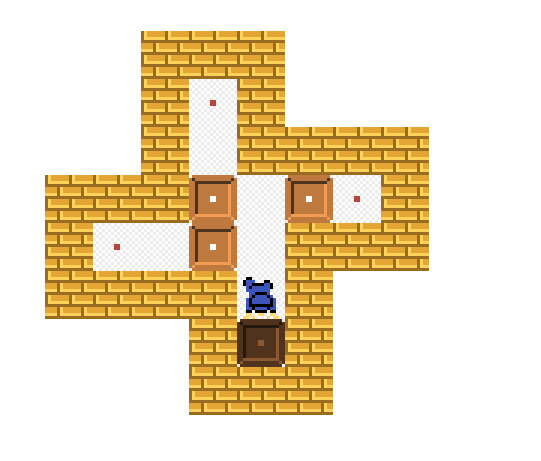
\includegraphics[width=7cm]{figures/sokoban}
    \caption{用于 WorldCoder 的 Sokoban~\citep{tang2024worldcoder}}\label{fig:sokoban}
\end{figure}

\begin{figure}
  \centering
    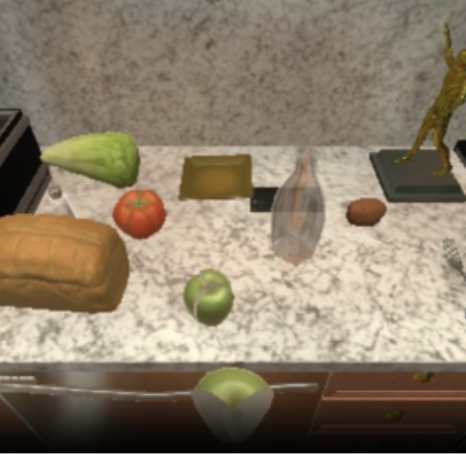
\includegraphics[width=6cm]{figures/alfworld}
    \caption{用于 WorldCoder 的 AlfWorld \citep{tang2024worldcoder}}\label{fig:alfworld}
\end{figure}

\paragraph{WorldCoder}
WorldCoder \citep{tang2024worldcoder} 同样旨在提高样本效率，但采用不同方法。它用可解释的 Python 代码生成动力学模型，也就是转移函数与奖励函数，再将其用于标准的基于模型的强化学习设计，以提高效率。生成的 Python 代码，比执行大语言模型推理更高效。WorldCoder 用于网格任务，例如图~\ref{fig:sokoban}~中的 Sokoban，以及家庭任务规划，例如图~\ref{fig:alfworld}~中的 AlfWorld。

\subsection{架构}
世界模型的目的是给观测赋予语义：动作会产生后果，而这一点可能是大语言模型与视觉语言模型的难点。某个像素何时属于可以行走的地板，从而限制 $y$ 方向运动；何时又属于阻挡前进的墙壁，从而限制 $x$ 方向运动？奖励函数提供反馈，说明哪些动作好、哪些不好。因此，世界模型架构通常采用强化学习设定，根据反馈奖励训练行动策略。我们可以把世界模型看作一个内部带有策略学习器的视觉语言模型。

WorldGPT、WebDreamer 与 WorldCoder 采用不同的世界模型架构，下面进一步讨论。

\begin{figure}
    \centering
    % 保留原始面板、实拍、示例与全部连线；仅以 TikZ 覆盖说明标签。
\begin{tikzpicture}
\node[anchor=south west,inner sep=0] (im) at (0,0) {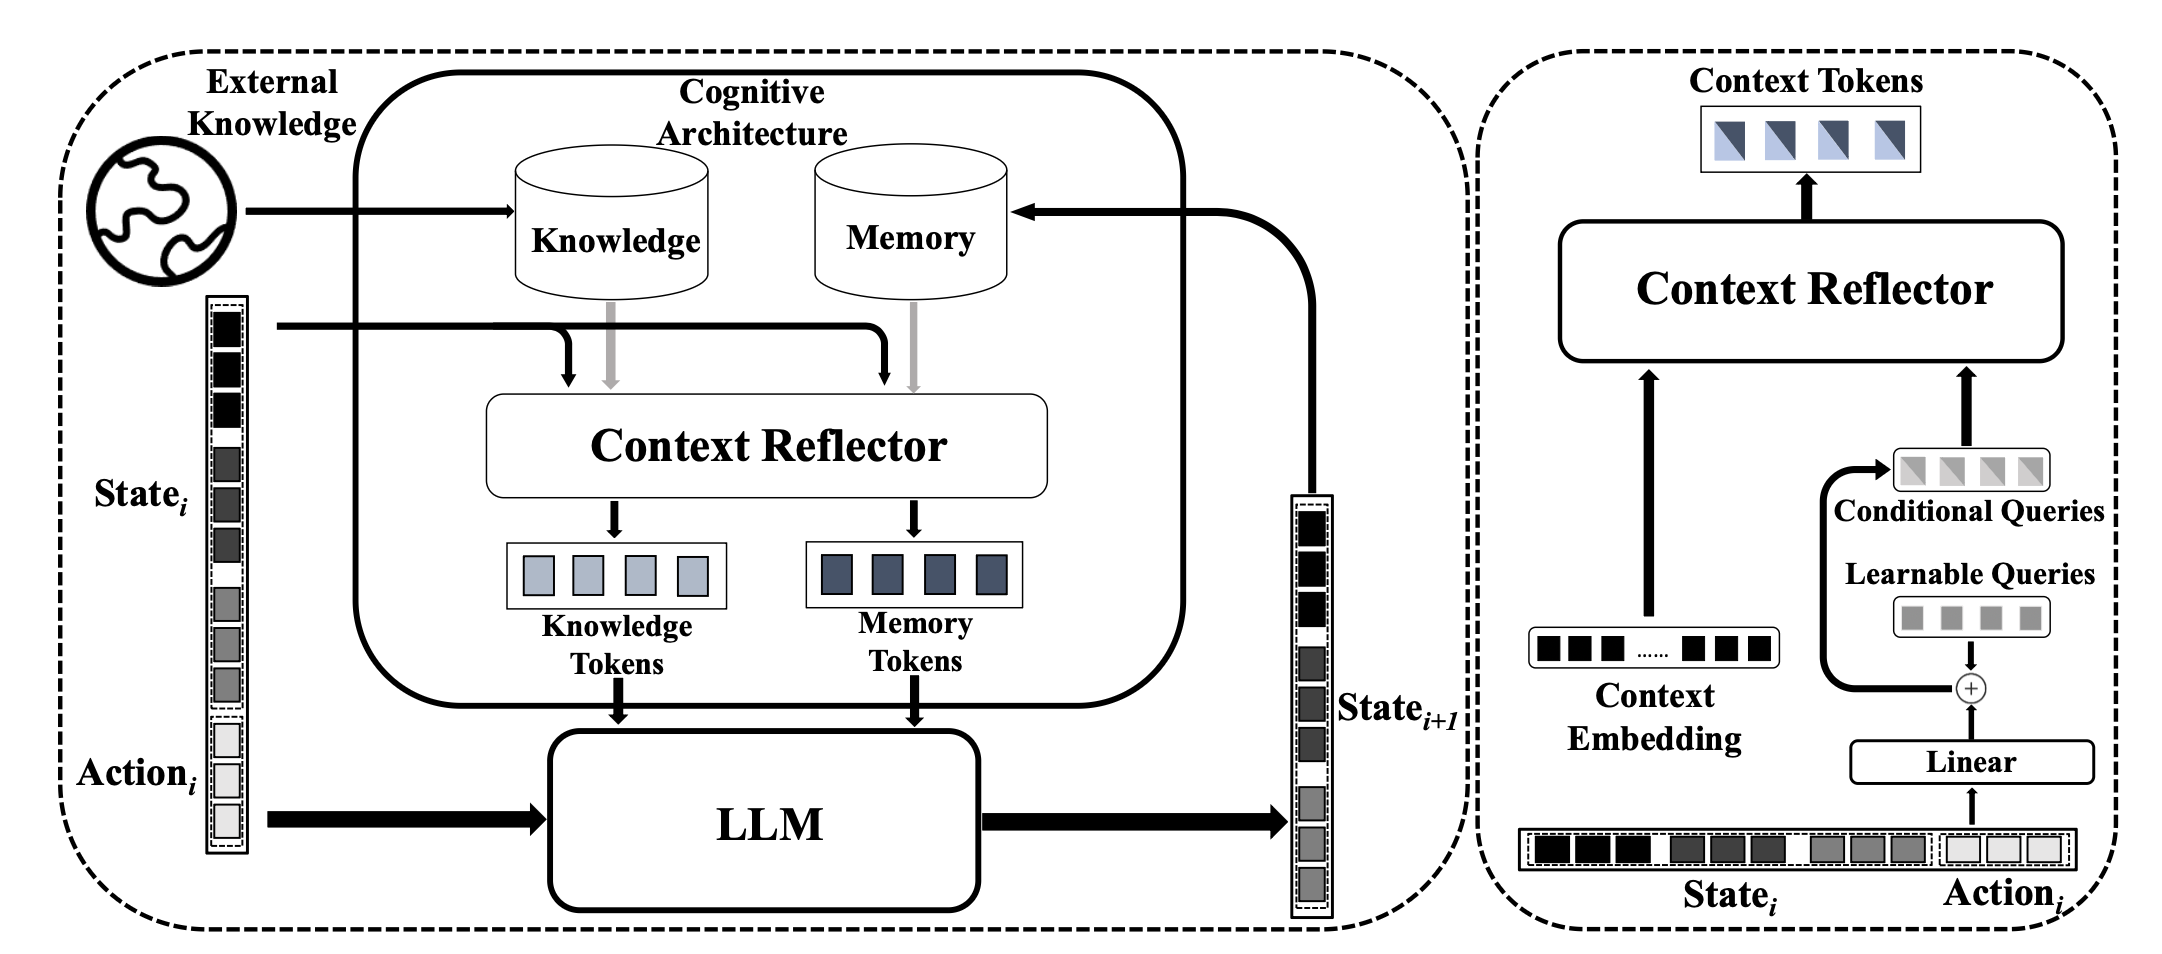
\includegraphics[width=\linewidth]{figures/worldgpt.png}};
\begin{scope}[x={(im.south east)},y={(im.north west)}]
\fill[white] (0.082500,0.850000) rectangle (0.167500,0.940000);
\node[align=center,inner sep=0pt,font=\fontsize{8.5}{9.5}\selectfont,text width=0.085000\linewidth,rotate=0] at (0.125000,0.895000) {外部\\知识};
\fill[white] (0.300293,0.838496) rectangle (0.411133,0.921460);
\node[align=center,inner sep=0pt,font=\fontsize{8.5}{9.5}\selectfont,text width=0.110840\linewidth,rotate=0] at (0.355713,0.879978) {认知架构};
\fill[white] (0.239000,0.723500) rectangle (0.329000,0.778500);
\node[align=center,inner sep=0pt,font=\fontsize{9}{10}\selectfont,text width=0.090000\linewidth,rotate=0] at (0.284000,0.751000) {知识};
\fill[white] (0.386000,0.725500) rectangle (0.466000,0.780500);
\node[align=center,inner sep=0pt,font=\fontsize{9}{10}\selectfont,text width=0.080000\linewidth,rotate=0] at (0.426000,0.753000) {记忆};
\fill[white] (0.242000,0.498000) rectangle (0.472000,0.566000);
\node[align=center,inner sep=0pt,font=\fontsize{10}{11}\selectfont,text width=0.230000\linewidth,rotate=0] at (0.357000,0.532000) {上下文反思器};
\fill[white] (0.238500,0.278000) rectangle (0.333500,0.366000);
\node[align=center,inner sep=0pt,font=\fontsize{8.5}{9.5}\selectfont,text width=0.095000\linewidth,rotate=0] at (0.286000,0.322000) {知识\\词元};
\fill[white] (0.380000,0.280000) rectangle (0.470000,0.368000);
\node[align=center,inner sep=0pt,font=\fontsize{8.5}{9.5}\selectfont,text width=0.090000\linewidth,rotate=0] at (0.425000,0.324000) {记忆\\词元};
\fill[white] (0.029000,0.454000) rectangle (0.099000,0.504000);
\node[align=center,inner sep=0pt,font=\fontsize{8}{9}\selectfont,text width=0.070000\linewidth,rotate=0] at (0.064000,0.479000) {状态$_i$};
\fill[white] (0.021500,0.158000) rectangle (0.096500,0.218000);
\node[align=center,inner sep=0pt,font=\fontsize{8}{9}\selectfont,text width=0.075000\linewidth,rotate=0] at (0.059000,0.188000) {动作$_i$};
\fill[white] (0.614000,0.232500) rectangle (0.678000,0.277500);
\node[align=center,inner sep=0pt,font=\fontsize{7.5}{8.5}\selectfont,text width=0.064000\linewidth,rotate=0] at (0.646000,0.255000) {状态$_{i+1}$};
\fill[white] (0.755000,0.889000) rectangle (0.913000,0.939000);
\node[align=center,inner sep=0pt,font=\fontsize{9}{10}\selectfont,text width=0.158000\linewidth,rotate=0] at (0.834000,0.914000) {上下文词元};
\fill[white] (0.743000,0.657500) rectangle (0.933000,0.722500);
\node[align=center,inner sep=0pt,font=\fontsize{10}{11}\selectfont,text width=0.190000\linewidth,rotate=0] at (0.838000,0.690000) {上下文反思器};
\fill[white] (0.845000,0.440000) rectangle (0.975000,0.480000);
\node[align=center,inner sep=0pt,font=\fontsize{8}{9}\selectfont,text width=0.130000\linewidth,rotate=0] at (0.910000,0.460000) {条件查询};
\fill[white] (0.844000,0.374000) rectangle (0.974000,0.414000);
\node[align=center,inner sep=0pt,font=\fontsize{8}{9}\selectfont,text width=0.130000\linewidth,rotate=0] at (0.909000,0.394000) {可学习查询};
\fill[white] (0.721500,0.191500) rectangle (0.826500,0.276500);
\node[align=center,inner sep=0pt,font=\fontsize{8.5}{9.5}\selectfont,text width=0.105000\linewidth,rotate=0] at (0.774000,0.234000) {上下文\\嵌入};
\fill[white] (0.871000,0.181500) rectangle (0.951000,0.214500);
\node[align=center,inner sep=0pt,font=\fontsize{8}{9}\selectfont,text width=0.080000\linewidth,rotate=0] at (0.911000,0.198000) {线性层};
\fill[white] (0.763500,0.039000) rectangle (0.838500,0.079000);
\node[align=center,inner sep=0pt,font=\fontsize{8}{9}\selectfont,text width=0.075000\linewidth,rotate=0] at (0.801000,0.059000) {状态$_i$};
\fill[white] (0.884766,0.026549) rectangle (0.989258,0.084071);
\node[align=center,inner sep=0pt,font=\fontsize{8}{9}\selectfont,text width=0.104492\linewidth,rotate=0] at (0.937012,0.055310) {动作$_i$};
\end{scope}
\end{tikzpicture}

    \caption{WorldGPT 架构 \citep{ge2024worldgpt}。}
    \label{fig:worldgpt}
\end{figure}

\paragraph{WorldGPT}
WorldGPT 基于标准大语言模型 Vicuna-7B-v0。\footnote{\url{https://huggingface.co/lmsys/vicuna-7b-v1.3}，\url{https://lmsys.org}}它遵循基于模型的强化学习方法，在潜在空间中进行推理。WorldGPT 的目标，是成为能够模拟现实世界动力学的模拟器，也就是强化学习中的转移函数与奖励函数。为此，它采用专门的架构，帮助合成多模态指令实例。其核心沿用常见的视觉语言模型架构，包含居中的大语言模型，以及多模态编码器与解码器。为了帮助模型合成多模态指令，又增加了一个认知架构，以支持专业化任务或长期任务。该架构加入记忆、知识检索与上下文反思，其中上下文反思建立在 Q-former 之上 \citep{li2023blip}。架构示意见图~\ref{fig:worldgpt}。

\paragraph{WebDreamer}
WebDreamer 面向网页交互，将大模型 Qwen-70B \citep{bai2025qwen2} 蒸馏为一个 7B 小模型。随后，小模型在真实网页世界中行动之前，先用作世界模型来模拟动作。它采用模型预测控制（model predictive control，MPC）作为规划方法 \citep{garcia1989model,schwenzer2021review}，决策网页动作，并在每个交互步骤重新规划。WebDreamer 将大语言模型同时用作世界模型与价值函数。大语言模型实现模拟函数 sim 与评分函数 score，见图~\ref{fig:webdreamer}。此外，沿用 \citep{koh2024tree} 的做法，大语言模型还用于生成候选动作。作者采用两个阶段：先采样排名靠前的 $k$ 个动作，再让大语言模型自行精炼，去掉不必要的动作，以供模拟。

\begin{figure}
    \centering
    % 完整转录原图伪代码；不增加算法编号，沿用原 figure 计数。
\begingroup
\algrenewcommand\algorithmicrequire{\textbf{输入：}}
\algrenewcommand\algorithmicensure{\textbf{输出：}}
\algrenewcommand\algorithmicwhile{\textbf{当}}
\algrenewcommand\algorithmicdo{\textbf{时}}
\algrenewcommand\algorithmicif{\textbf{如果}}
\algrenewcommand\algorithmicthen{\textbf{则}}
\algrenewcommand\algorithmicend{\textbf{结束}}
\algrenewtext{EndWhile}{\textbf{结束循环}}
\algrenewtext{EndIf}{\textbf{结束判断}}
\begin{minipage}{.94\linewidth}
\hrule\smallskip
\begin{algorithmic}
\Require 指令 $I$；初始观测 $o_0$
\Ensure 动作序列 $a_0,a_1,\ldots,a_T$
\State $t\gets 0$;
\While{\texttt{True}}
  \State $\mathcal{A}_t\gets\texttt{get\_candidate}(I,o_t)$;
  \State $\mathcal{A}'_t\gets\texttt{self\_refine}(\mathcal{A}_t)$;
  \State $a_t=\arg\max_{a\in\mathcal{A}'_t}\texttt{score}(\texttt{sim}(o_t,a))$;
  \State $o_{t+1}\gets\texttt{execute}(a_t)$;
  \State $t\gets t+1$;
  \If{$\texttt{termination\_check}()=\texttt{True}$}
    \State \textbf{跳出循环};
  \EndIf
\EndWhile
\end{algorithmic}
\smallskip\hrule
\end{minipage}
\endgroup

    \caption{WebDreamer 伪代码：用大语言模型实现 score 与 sim 函数 \citep{gu2024your}。}
    \label{fig:webdreamer}
\end{figure}

\paragraph{WorldCoder}
\begin{figure}
    \centering
    % 原图的全部方向关系保留；框中的 Python 标识符与代码保持英文。
\resizebox{\linewidth}{!}{%
\begin{tikzpicture}[font=\small,flow/.style={-{Stealth[length=2mm]},line width=.8pt},box/.style={draw,fill=white,align=center,inner sep=4pt}]
\node[circle,draw,minimum size=1.3cm] (world) at (0,0) {世界};
\node[align=center] (feedback) at (2.2,1.3) {状态、\\奖励、目标};
\node[box] (plan) at (3.8,0) {规划器};
\node[box,fill=black,text=white,font=\ttfamily\footnotesize,align=left] (program) at (7.6,0) {\# world\_model.py\\def update(state, action, goal):\\\quad ...............................\\\quad return new\_state, reward};
\node[box] (llm) at (11.7,0) {LLM};
\node[box,rounded corners=5pt] (replay) at (13.6,0) {经验回放\\缓冲区};
\draw[flow] (world.north) to[out=70,in=180] (feedback.west);
\draw[flow] (feedback.east) to[out=0,in=90] (plan.north);
\draw[flow] (feedback.east) .. controls (10.5,1.5) and (13.6,1.6) .. (replay.north);
\draw[flow] (plan.south) .. controls (3,-1.0) and (.5,-1.2) .. node[below] {动作} (world.south);
\draw[flow] (program.west) -- (plan.east);
\draw[<->,>=Stealth,line width=.8pt] (program.east) -- (llm.west);
\draw[flow] (replay.west) -- (llm.east);
\draw[flow] (plan.south) .. controls (5,-1.2) and (13.6,-1.2) .. (replay.south);
\end{tikzpicture}%
}

    \caption{WorldCoder 架构 \citep{tang2024worldcoder}。}
    \label{fig:worldcoder}
\end{figure}
WorldCoder 是一个基于模型的智能体，构建 Python 程序来表示自身的世界知识。它用可执行 Python 代码创建世界的转移函数，见图~\ref{fig:worldcoder}。WorldCoder 使用程序合成（program synthesis）。在强化学习中，问题被形式化为马尔可夫决策过程，包括状态表示 $S$、动作函数 $A$、转移函数 $T$ 与奖励函数 $R$，见第~\ref{sec:mbrl}~节。WorldCoder 使用大语言模型，为任务生成动作函数、转移函数、奖励函数以及状态表示的 Python 代码，再将其用于基于模型的强化学习方法。这些代码通过反复的自我调试与精炼进行检查、改进 \citep{chen2023teaching}，见第~\ref{sec:selfdebug}~节。这个过程不断重复，直到程序产生正确输出。

需要注意，WorldCoder 学到的是符号模型，转移函数表示为计算机代码；通常的深度强化学习则使用神经网络模型。WorldCoder 在推理阶段效率较高，因为不需要调用大语言模型、对大型网络做前向传播，只需要解释执行转移函数与奖励函数的 Python 代码。

通常，基于模型的大语言模型方法让大语言模型{\em 模拟}世界；WorldCoder 则让大语言模型{\em 构建}世界模拟，留待后续执行。在推理阶段，Python 解释器执行转移函数；ReAct 则由大语言模型对世界状态进行推理。对于规划问题，符号方法更合适，因为大语言模型在推理过程中难以进行规划，见第~\ref{sec:knowing}~节。

\subsection{学习算法}
下面讨论这些不同方法采用的预训练与微调算法。

\paragraph{WorldGPT}
WorldGPT 通过在不同领域的数百万段视频上预训练与微调，获得对世界动力学的理解。其基础大语言模型采用 Vicuna-7B-v0。预训练使用以语言为中心的编码器，得到多模态状态的统一表示。为了进行多模态解码，在大语言模型词表中加入特殊词元。训练从单模态开始，逐步过渡到跨模态。微调采用专门的认知强化架构，以及一个包含来自超过一千万段视频的细粒度序贯状态转移样本标注的数据集。如前所述，认知架构由记忆、知识检索与上下文反思组成。智能体通过在合成多模态指令数据上微调，获得专业化知识。

\paragraph{WebDreamer} WebDreamer 旨在学习适合基于模型的强化学习的动力学。首先，用预训练视觉语言模型 Qwen-2-VL \citep{wang2024qwen2} 初始化 Dreamer-7B，再在 310 万个交互样例上进一步微调。数据合成流程包含两部分：(1) 在网页上随机游走，模型自主通过输入搜索文字、点击等动作与网页交互；(2) 合成，由 Qwen2-VL-72B 根据动作前后的视觉快照，生成状态变化的文字描述。WebDreamer 针对每个动作，在有限时域内模拟可能的未来状态，遵循模型预测控制方法，重新规划并重新训练；这是一种用于工程与控制问题、进行自适应重新训练的强化学习方法。

\paragraph{WorldCoder}
WorldCoder 通过程序合成，学习构建用于计算下一世界状态的转移函数。随后，它使用代码实现的世界模型，执行规划动作。首先，通过随机探索初始化环境交互数据集；然后，利用程序合成算法更新世界模型、生成代码，再进行规划。可以使用不同规划器，从简单领域中的深度受限价值迭代，到复杂领域中的蒙特卡洛树搜索（Monte Carlo tree search，MCTS）\citep{browne2012survey}。

\subsection{结果}
现在来看这三种方法的结果。

\paragraph{WorldGPT} WorldGPT 使用多模态状态转移预测基准测试评估。模型表现有效，能够准确理解与预测现实世界中复杂厨房和烹饪场景的动力学。

系统也作为世界模拟器接受评估，展现了泛化到陌生领域的能力。在一项实验中，WorldGPT 在音视频问答任务上的速度，比传统的基于扩散的方法快 30 倍 \citep{ge2024worldgpt}。

\paragraph{WebDreamer} WebDreamer 同样表现良好。据报告，它在网页交互任务上的表现超过 GPT-4o。相对于反应式基线，报告显示了显著的性能提升，而效率达到树搜索的 4—5 倍。WebDreamer 在沙箱环境 VisualWebArena，以及 Online-Mind2Web、Mind2Web-Live 等真实网站上，都取得良好表现；在真实网站上，树搜索方法很难实现与部署。此外，在在线基准测试中，采用 Dreamer-7B 的方法，取得了可与 GPT-4o 相比的性能。在真实网站上，WebDreamer 相对于反应式基线，分别取得 42\% 与 24\% 的相对提升。

\paragraph{WorldCoder}
WorldCoder 的结果在网格世界与 AlfWorld 任务规划上报告。与无模型强化学习相比，WorldCoder 的样本效率更高；与尝试用大语言模型进行上下文规划的 ReAct 式智能体相比，其计算效率也更高。

由大语言模型以计算机代码生成世界知识，具有若干优点。模型内含的先验世界知识能够改善代码生成，因为已发表问题的现成解法，很可能已经在预训练中出现过。通过复用旧程序片段，代码也能够在任务间迁移。此外，结果对人类可读，人们可以通过阅读生成代码，检查其中的世界知识。

虽然 WorldCoder 对规划问题很有潜力，但它也受到规划问题固有计算难度的限制。专用求解器难以解决的问题实例，对 WorldCoder 求解器同样困难。大语言模型生成的转移函数，不太可能优于人类专家研究者设计的转移函数。

目前，合成代码的目标，是复现转移函数与奖励函数。未来，自我反思与元学习方法可能进一步改善性能。

\subsection{*基于模型的强化学习}\label{sec:mbrl}

世界模型已经成功用于智能体大语言模型。关于基于模型的强化学习中的世界模型，也已有大量文献。在本章末尾，我们将简要概述这一领域，为理解世界模型在大语言模型中的用途提供更多背景。

一个有影响力的早期方法是 Dyna \citep{sutton1991dyna}。近期有影响力的工作包括 \citep{ha2018world,hafner2020mastering}。两篇现代综述是 \citet{moerland2023model,plaat2023high}。

在强化学习中，智能体对环境中执行的动作所获奖励进行采样，学习如何在环境中行动。

\begin{figure}
  \begin{center}
    \input figures/rl
    \caption{标准强化学习循环。智能体根据环境反馈的奖励 $r$，学习由参数 $\theta$ 表征的策略 $\pi_\theta$。\citep{sutton2018reinforcement}}\label{fig:rl7b}
  \end{center}
\end{figure}

\subsubsection{无模型强化学习}
在通常的强化学习中，以无模型方式学习最优智能体策略：直接通过与环境交互，学习所有状态下的最佳动作，见图~\ref{fig:rl7b}，而不借助额外的环境模型。通常的强化学习形式化为包含四个函数 $\{S, T, A, R\}$ 的马尔可夫决策过程：函数 $S(o)\rightarrow s$ 根据观测 $o$ 表示系统状态；函数 $T(s,a)\rightarrow s'$ 根据动作使一个状态转移到下一个状态；函数 $A(s)\rightarrow a$ 返回某个状态下的动作；函数 $R(s)\rightarrow r$ 为状态赋予一个正或负的奖励值。强化学习的目标，是利用马尔可夫决策过程学习最优策略 $\pi^*(s)\rightarrow a^*$，即为该过程可能处于的每个状态，返回最佳动作的函数。因此，强化学习问题由函数 $S$、$T$、$A$ 与 $R$ 构成，智能体的目标，是找到具有最高期望累积奖励的最优策略 $\pi^*(s)$。智能体不能直接访问位于环境中的函数 $T$ 与 $R$。
通常的无模型强化学习，也称为{\em 直接}强化学习。直接方法天然具有较高的样本复杂度：改进策略需要采样，而大型马尔可夫决策过程需要大量样本，才能使策略改进过程收敛，见图~\ref{fig:rl7b}。

\begin{figure}[ht]
  \begin{center}
    \input figures/mbrl
    \caption{基于模型的强化学习：环境反馈同时用于改进策略 $\pi$ 与本地动力学模型 $\hat{M}=(\hat{T},\hat{R})$；也可以从该模型采样，学习策略 $\pi$，即{\em 规划}。}\label{fig:mbrl}
  \end{center}
\end{figure}

\subsubsection{基于模型的强化学习}
在直接强化学习中，采样得到的信息不会被智能体保留，而是被遗忘，每次改进策略都需要新样本。智能体与外部环境交互往往代价高昂，例如现实世界中行动的机器人，其关节会磨损。这时，寻找降低样本复杂度的方式就很有价值。我们应当尝试在减少环境采样的同时改进策略。

一个直接的想法是，不丢弃样本，而是把它们存入缓冲区，再从这些旧交互结果中采样。稍进一步，则可以为环境动力学训练一个{\em 本地代理模型（local surrogate model）} $M=(\hat{T}, \hat{R})$。训练好这个本地动力学模型后，除了昂贵地对环境采样，也能够以较低成本对模型采样，见图~\ref{fig:mbrl}。

这些属于间接方法：在后面这些由智能体构建本地动力学模型的方法中，策略通过本地模型，间接地从环境中学得。

使用本地动力学模型的方法，称为基于模型的强化学习。动力学模型包含智能体本地估计的 $\hat{T}$ 与 $\hat{R}$，即对只有环境知道的真实 $T$ 与 $R$ 的估计。基于模型的强化学习已经在围棋 \citep{silver2016mastering}、Diplomacy \citep{meta2022human}、StarCraft \citep{vinyals2019grandmaster} 等应用中取得成功，并展现了跨领域学习能力 \citep{hafner2020mastering}。

基于模型的强化学习还联系着符号人工智能中的经典领域——{\em 规划}。规划利用高效的潜在表示向未来展望，模拟不同的可能世界，无须在真实世界中行动。

\subsubsection{降维}
在深度的基于模型的强化学习中，本地动力学模型也称为世界模型 \citep{ha2018world}。在这一语境下，世界模型把高维观测空间缩减为低维状态空间与奖励空间，随后供基于模型的强化学习方法使用，高效改进策略函数。
其背后的思想是，大多数高维环境中都存在不太重要的元素。例如，电子游戏背景中从不移动的树木，与智能体动作的价值可能几乎无关。目标是抽象掉输入空间中的这些不重要元素，降低状态空间的有效维数。

\subsubsection{联合嵌入预测架构}
联合嵌入预测架构（joint embedding predictive architecture，JEPA）由 \citet{lecun2022path} 提出，并在 \citet{assran2023self} 中进一步完善。JEPA 的目标，是在抽象、压缩的表示，也就是潜在空间中预测未来状态，而不是重建原始感官细节或像素。这与基于模型的强化学习中世界模型的降维目标相似。基于模型的强化学习在奖励监督下学习本地转移模型，而 JEPA 是一种自监督表示学习框架。
JEPA 通过观看视频或图像这样的自监督观测进行训练，把上下文嵌入映射为目标嵌入，不使用奖励或显式动作。基于模型的强化学习则显式纳入动作、奖励与控制优化，以最大化回报 \citep{lim2026jedi}。JEPA 与强化学习关系密切：它可以作为强化学习或规划算法的感知引擎，也就是世界模型，例如用来引导机器人控制 \citep{destrade2025value}。

\subsubsection{智能体世界模型}
在基于模型的强化学习中，大语言模型有两种不同用法。第一，可以把预训练的、静态的大语言模型用作世界模型 $(\hat{T}, \hat{R})$，服务于基于模型的强化学习，即 LLM4MBRL。这类方法通常采用树搜索或蒙特卡洛树搜索进行规划。在这种方法中，大语言模型帮助强化学习。

另一种方式，是使用基于模型等强化学习设定，通过世界交互反馈训练大语言模型世界模型，即 MBRL4LLM。此时，大语言模型具有了适应性，可以通过自适应控制框架实现，也可以像视觉语言动作模型一样，对模型本身进行后训练。这种方法也称为智能体世界模型，有望帮助智能体更好地理解环境，以更加符合现实的方式行动。在这种方法中，强化学习帮助智能体语言建模。这是一个活跃研究方向，例如可参阅 \citet{zuo2026qwen} 及其引用文献。\footnote{强化学习与语言建模之间还有第三种联系：在大语言模型训练流程{\em 内部}，无模型强化学习也用于微调，例如基于人类反馈的强化学习与可验证奖励强化学习。}

\section{结语}

Transformer 可以在词元化语言数据上训练，也可以在其他词元化数据上训练。本章介绍了用于不同模态的不同模型架构。虽然架构差异很大，但大多数模型都以 Transformer 为基础，人们也为种类丰富得令人惊讶的模态设计了词元化方法。回顾这些模型，可以看到它们的共同之处：
\begin{itemize}
    \item 大语言模型是在{\em 词元化自然语言}上预训练的 Transformer。
    \item 视觉语言模型由在{\em 词元化视觉数据}上训练的 Transformer，也可以是扩散模型或卷积网络，以及在{\em 词元化自然语言}上训练的 Transformer 组成，二者的嵌入在联合解码器中汇合。
    \item 决策 Transformer 在决策路径的{\em 词元化 $(s,a,r)$ 回合}上训练，见第~\ref{sec:decisions}~节。
    \item 视觉语言动作模型由视觉语言架构组成，同时在机器人动作的{\em 词元化 $(s,a,r)$ 回合}上训练。
    \item 世界模型由视觉语言架构组成，同时在现实世界动作或决策的{\em 词元化 $(s,a,r)$ 回合}上训练。
\end{itemize}
还有其他一些模型，本章并未讨论。例如，大型音乐模型（large music model，LMM）是在词元化音乐序列上预训练的 Transformer；这些序列既可以是乐谱这样的符号音乐，也可以是音轨 \citep{yuan2025yue}。

本章专门讨论面向智能体的先进模型，介绍了在视觉与动作数据上预训练、微调的语言模型。这些模型能够理解更多世界知识，使智能体取得令人印象深刻的泛化结果。我们看到，最初作为语言模型的大语言模型，正在成为世界模型；这个术语借自基于模型的强化学习领域。

到这里，不妨回顾一下已经介绍的内容。本书第一部解释了如何通过自指式方式，为{\em 语言}任务{\em 预训练}模型。随后，第~\ref{chap:reasoning}~章解释了{\em 上下文学习}如何涌现，以及如何用它在推理阶段进行{\em 多步推理}与自我反思。本章讨论了通过{\em 预训练}与{\em 微调}，得到环境的{\em 多模态世界}模型。预训练的语言能力、推理阶段的推理能力，以及微调所得的世界模型，共同使智能体越来越能够为用户在世界中智能行动、完成任务。

现在，我们已经讨论了许多不同模态与训练方法。下一章将退后一步，思考智能体如何在自己赖以学习的世界中行动的同时，保持稳定的学习。

\bibliographystyle{plainnat}
\bibliography{agenticbook,refs,case,synthetic}
